% =====================================================================
%  LMECA2323 - Turbomachinery Project
%  Characterization of a high-pressure turbine stage
%  Modular report.  Compile with:  latexmk -pdf Report.tex
% =====================================================================
\documentclass[11pt,a4paper]{report}

\usepackage[utf8]{inputenc}
\usepackage[T1]{fontenc}
\usepackage[margin=2.5cm]{geometry}
\usepackage{graphicx}
\usepackage{grffile}   % allow spaces / extra dots / parentheses in image filenames
\usepackage{amsmath,amssymb}
\usepackage{booktabs}
\usepackage{array}
\usepackage{caption}
\usepackage{subcaption}
\usepackage{float}
\usepackage{siunitx}
\usepackage{fancyhdr}
\usepackage{xcolor}
\usepackage[hidelinks]{hyperref}
\usepackage{wrapfig}
\graphicspath{{Figures/}}

% ---- running header / footer (mimics the reference report) ----------
\pagestyle{fancy}
\fancyhf{}
\fancyhead[L]{\small\itshape High-pressure stage turbine design}
\fancyfoot[R]{\small Page | \thepage}
\renewcommand{\headrulewidth}{1.0pt}
\renewcommand{\footrulewidth}{0.4pt}

\captionsetup{font=small,labelfont=bf}
\setlength{\parskip}{0.5em}
\setlength{\parindent}{0pt}

% degree symbol used throughout the chapters
\newcommand{\degr}{\ensuremath{^\circ}}

\begin{document}

% ------------------------------- Title page -------------------------------
\begin{titlepage}
\thispagestyle{empty}
\begin{center}

\begin{minipage}{0.45\textwidth}
    \raggedright
    
\includegraphics[height=1.6cm]{UCLouvain_logo.svg.png}
\end{minipage}
\hfill
\begin{minipage}{0.45\textwidth}
    \raggedleft
    
\includegraphics[height=1.6cm]{epl.png}
\end{minipage}

\vspace{2.0cm}
\rule{\textwidth}{0.4pt}\\[0.6cm]

{\LARGE \textbf{LMECA2323 -- Turbomachinery}}\\[0.4cm]
{\LARGE \textbf{Project -- 2026}}\\[0.8cm]
{\Large Characterization of a high-pressure turbine stage}\\[0.3cm]
{\Large for an industrial power production gas turbine}\\[0.4cm]

\rule{\textwidth}{0.4pt}

\vspace{1.6cm}

{\textbf{Professors}}\\[0.15cm]
L. Bricteux\\
S. Lavagnoli\\[0.6cm]

{\textbf{Teaching Assistants}}\\[0.15cm]
Ir. Romain Debroyer\\
Ir. Antoine Verhaeghe\\[1.0cm]

{\textbf{Student:}}\\[0.15cm]
RANI, Sanjana

\vfill
{\small 31-05-2023}

\end{center}
\end{titlepage}


\pagenumbering{roman}
\tableofcontents
\listoffigures
\listoftables
\clearpage
\pagenumbering{arabic}

% ------------------------------- Chapter 1 -------------------------------
\chapter{Introduction}

A turbomachine produces or absorbs energy through a change of enthalpy in a
continuously flowing stream, transferring work through a rotating shaft. In a
gas turbine the turbine extracts work from the hot combustion products by
expansion: the flow accelerates at the expense of pressure, and a large part of
the extracted power is used to drive the compressor through the shaft, the
remainder being the useful (net) output.

Designing a turbine stage couples thermodynamics, kinematics (velocity
triangles), annulus geometry and mechanical constraints~\cite{dixon}. The
procedure followed in this work is the classical three-step chain of preliminary
design:

\begin{itemize}
    \item \textbf{1-D mean-line design} -- thermodynamic and velocity-triangle
          analysis on the mean streamline;
    \item \textbf{Rotor-blade design} -- conversion of the flow angles into a
          blade profile (chord, stagger, pitch, blade count);
    \item \textbf{CFD evaluation} -- meshing and RANS solution of the resulting
          cascade to verify the loading and exit flow.
\end{itemize}

\begin{wrapfigure}{r}{0.55\textwidth}
    \centering
    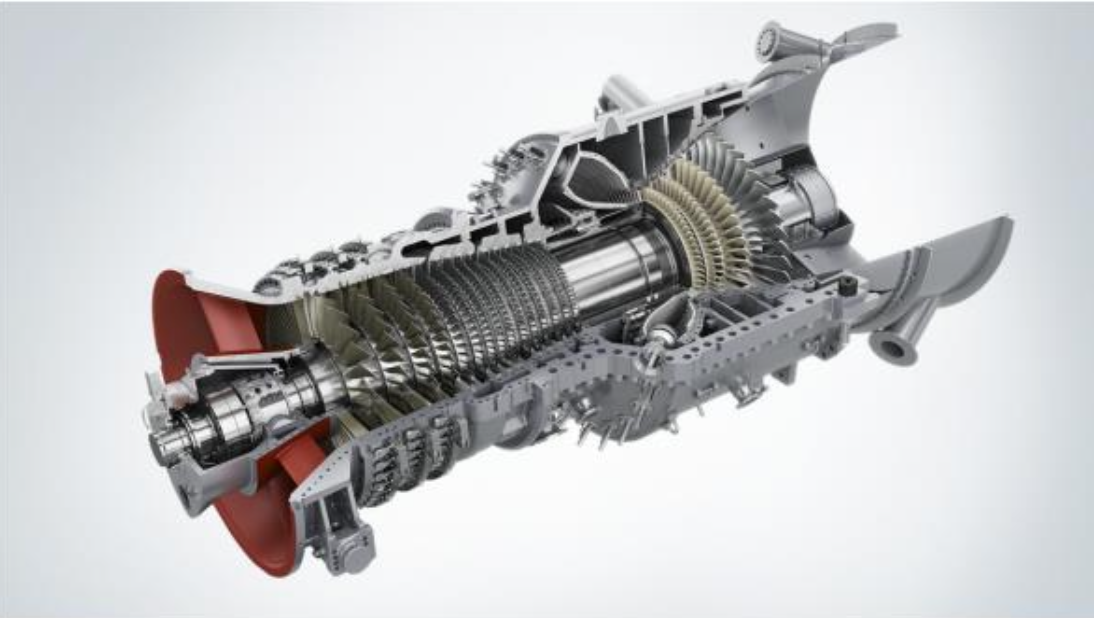
\includegraphics[width=\linewidth]{engine.png}
    \caption{Industrial gas turbine of the SGT5-4000F class (cutaway).}
    \label{fig:engine}
\end{wrapfigure}

These steps are not executed once and in isolation: the design coefficients
(stage loading $\psi$, flow coefficient $\phi$ and degree of reaction $r$) are
iterated until the resulting stage satisfies a set of aerodynamic and mechanical
design guidelines. This report focuses on the \textbf{first stage} of a
four-stage high-pressure turbine sized for the conditions of an F-class
industrial gas turbine (representative of the Siemens SGT5-4000F), delivering
\SI{330}{MW} of shaft power at a mass flow of \SI{750}{kg/s}.




The whole design chain has been implemented in Python (the accompanying
notebook): the mean-line solver, the ParaBlade-based blade
construction~\cite{parablade} and the GMSH~\cite{gmsh}\,+\,SU2~\cite{su2} cascade
CFD. All numerical results, tables and figures in this report are produced
directly by that code.

% ------------------------------- Chapter 2 -------------------------------
\chapter{1-D Mean-Line Design}

The 1-D mean-line design is the simplified modelling strategy used in the early
stages of turbine design. The flow is assumed axisymmetric and is averaged along
the radial direction, so that the whole stage is represented by the conditions on
the mean streamline. With this simplification the stage power, efficiency and
blade loading can be evaluated quickly and the design coefficients iterated.

The stage is divided into three stations: station~1 (stator inlet), station~2
(stator exit / rotor inlet) and station~3 (rotor exit).

% =====================================================================
\section{Input Data}

The following quantities are imposed by the project statement:

\begin{itemize}
    \item Working fluid: calorically perfect gas, $\gamma = 4/3 \approx 1.33$,
          $R = \SI{287}{J/kg/K}$.
    \item Turbine mass flow $\dot m = \SI{750}{kg/s}$; fuel-to-air ratio
          $f_{ar}=0.025$.
    \item Stage (extracted) shaft power $P = \SI{330}{MW}$ (the turbine also
          drives the compressor).
    \item Overall compressor pressure ratio $\Pi_C = 20$.
    \item Compressor admission $T_{adm} = \SI{15}{\degreeCelsius}$,
          $P_{adm} = \SI{101325}{Pa}$, isentropic efficiency $\eta_{is,C}=0.92$.
    \item Combustion-chamber Mach number $M_{comb}=0.15$.
    \item Turbine inlet static temperature (F-class) $TIT = \SI{1400}{\degreeCelsius}$.
    \item Inlet yaw angle $\alpha_1 = 0\degr$ (fully axial); rotational speed
          $N_{rot}=\SI{3000}{rpm}$ (synchronous generator).
    \item Blade peripheral speed limited to $U_m = \omega R_m \le \SI{350}{m/s}$;
          mechanical constraint $AN^2 < \SI{3e7}{m^2\,rpm^2}$.
    \item Constant mean radius $R_{mean}$ across the stage; fixed blading
          efficiencies $\eta_{S,R}=0.90$.
\end{itemize}

% =====================================================================
\section{Design Procedure}

\subsection{Inlet Condition Calculations}

The specific heats are obtained from $\gamma$ and $R$:
\begin{equation}
    c_p = \frac{\gamma R}{\gamma-1} = \SI{1156.70}{J/kg/K},\qquad
    c_v = \frac{R}{\gamma-1} = \SI{869.70}{J/kg/K}.
\end{equation}

Only air flows through the compressor, so its mass flow differs from the turbine:
\begin{equation}
    \dot m_c = \frac{\dot m_T}{1.025} = \SI{731.71}{kg/s}.
\end{equation}
With $\gamma_C = 1.4$ for the compressor, the absorbed compressor power is
\begin{equation}
    P_c = \frac{1}{\eta_{is}\,\eta_m}\,\dot m_c\,c_{p,C}\,T_{adm}
          \left[\Pi_C^{\frac{\gamma_C-1}{\gamma_C}}-1\right] = \SI{327.82}{MW},
\end{equation}
taking a mechanical efficiency $\eta_m = 0.95$. The compressor exit (turbine
inlet) static pressure follows from the pressure ratio,
\begin{equation}
    P_1 = \Pi_C \, P_{adm} = \SI{2026500}{Pa}.
\end{equation}
The turbine inlet stagnation properties are obtained from the combustion-chamber
Mach number:
\begin{align}
    P_{01} &= P_1\left(1+\tfrac{\gamma-1}{2}M_{comb}^2\right)^{\frac{\gamma}{\gamma-1}}
            = \SI{2056992}{Pa},\\
    T_{01} &= T_1\left(1+\tfrac{\gamma-1}{2}M_{comb}^2\right)
            = \SI{1679.21}{K},
\end{align}
with $T_1 = TIT = \SI{1673}{K}$.

\subsection{Required \texorpdfstring{$P_3$}{P3} Calculations}

The total power to be produced by the four-stage turbine is the sum of the net
shaft power and the compressor power, so the power per stage is
\begin{equation}
    P_{stage} = \frac{P + P_c}{4} = \SI{164.46}{MW}.
\end{equation}
The corresponding real specific work and isentropic enthalpy drop
(with $\eta_{TT}=0.87$) are
\begin{equation}
    \Delta H_{real} = \frac{P_{stage}}{\dot m} = \SI{219.27}{kJ/kg},\qquad
    \Delta H_{is} = \frac{\Delta H_{real}}{\eta_{TT}} = \SI{243.64}{kJ/kg}.
\end{equation}
The isentropic exit stagnation state and stage pressure ratio are
\begin{equation}
    T_{03,is} = T_{01}-\frac{\Delta H_{is}}{c_p} = \SI{1468.58}{K},\quad
    P_{03,is} = \SI{1198493}{Pa},\quad
    \Pi_{TT,is} = \frac{P_{01}}{P_{03,is}} \approx 1.72 .
\end{equation}
Assuming an exit Mach number $M_3 = 0.3$ (within the recommended $0.3$--$0.4$
band) closes the static exit state and gives a first estimate of $P_3$, which is
later refined by the iteration of Section~\ref{sec:enth}.

\subsection{Assumptions of Design Parameters}

Three coefficients are chosen and iterated to meet the design guidelines:

\paragraph{Stage loading $\psi = \Delta H_{real}/U^2$.}
For a high-pressure stage $\psi$ is typically $1.5$--$2$. It controls the width
of the velocity triangles, the turning and the exit Mach number. Fixing
$\psi = 1.8$ gives a blade speed
\begin{equation}
    U_m = \sqrt{\frac{\Delta H_{real}}{\psi}} = \SI{349.03}{m/s},
\end{equation}
just within the \SI{350}{m/s} mechanical limit.

\paragraph{Flow coefficient $\phi = V_x/U$.}
The flow coefficient sets the height of the velocity triangles. Using a Smith
chart~\cite{smith} at the chosen efficiency and $\psi$, a value $\phi = 0.5$ is
selected, giving an axial velocity $V_x = \SI{174.5}{m/s}$.

\paragraph{Degree of reaction $r = (h_2-h_3)/(h_1-h_3)$.}
For a cooled high-pressure stage the reaction is kept low, $0.35$--$0.5$; here
$r = 0.35$ is adopted.

% =====================================================================
\section{Thermodynamic Quantities}
\label{sec:thermo}

With the inlet state and the three coefficients fixed, the thermodynamic and
kinematic quantities are computed at every station. Station~2 follows from the
stator expansion ($V_{x2}=U\phi$, $P_2 = r(P_1-P_3)+P_3$, stator efficiency
$\eta_S$); the relative frame ($W_2$, $\beta_2$, $T_{02R}$, $P_{02R}$) is then
formed, and the rotor exit (station~3) is obtained from the relative isentropic
expansion to $P_3$ with rotor efficiency $\eta_R$. Table~\ref{tab:stations}
collects the converged values.

\begin{table}[H]
\centering
\caption{Thermodynamic and kinematic quantities at the three stations.}
\label{tab:stations}
\small
\begin{tabular}{l r r r}
\toprule
\textbf{Quantity} & \textbf{Station 1} & \textbf{Station 2} & \textbf{Station 3}\\
\midrule
Static pressure $P$ [Pa]            & 2026500 & 1428997 & 1107265 \\
Total pressure (abs.) $P_0$ [Pa]    & 2056992 & 1954202 & 1166813 \\
Rel. total pressure $P_{0R}$ [Pa]   & --      & 1521338 & 1472070 \\
Static temperature $T$ [K]          & 1673.0  & 1553.7  & 1470.4 \\
Total temperature (abs.) $T_0$ [K]  & 1679.2  & 1679.2  & 1489.6 \\
Rel. total temperature $T_{0R}$ [K] & --      & 1578.1  & 1578.1 \\
Absolute velocity $V$ [m/s]         & 174.5   & 538.8   & 211.0 \\
Axial velocity $V_x$ [m/s]          & 174.5   & 174.5   & 174.5 \\
Tangential velocity $V_u$ [m/s]     & 0.0     & 509.7   & 118.5 \\
Relative velocity $W$ [m/s]         & --      & 237.2   & 499.1 \\
Yaw angle $\alpha$ [\degr]          & 0.00    & 71.10   & 34.18 \\
Relative angle $\beta$ [\degr]      & --      & 42.64   & 69.53 \\
Absolute Mach $M$ [-]               & 0.22    & 0.70    & 0.30 \\
Relative Mach $M_w$ [-]             & --      & 0.31    & 0.67 \\
\bottomrule
\end{tabular}
\end{table}

The stator-exit Mach $M_2 = 0.70$ and the relative exit Mach $M_{w3}=0.67$ are
consistent with a low-reaction high-pressure stage in which the bulk of the
acceleration occurs in the stator.

% =====================================================================
\section{Velocity Triangles}

The velocity triangles at stations~2 and~3 are built from the blade speed $U$,
the absolute velocity $V$ and the relative velocity $W$, together with the flow
angle $\alpha$ and the blade angle $\beta$. They are plotted in
Fig.~\ref{fig:tri} and summarised in Table~\ref{tab:tri}.

\begin{figure}[H]
\centering
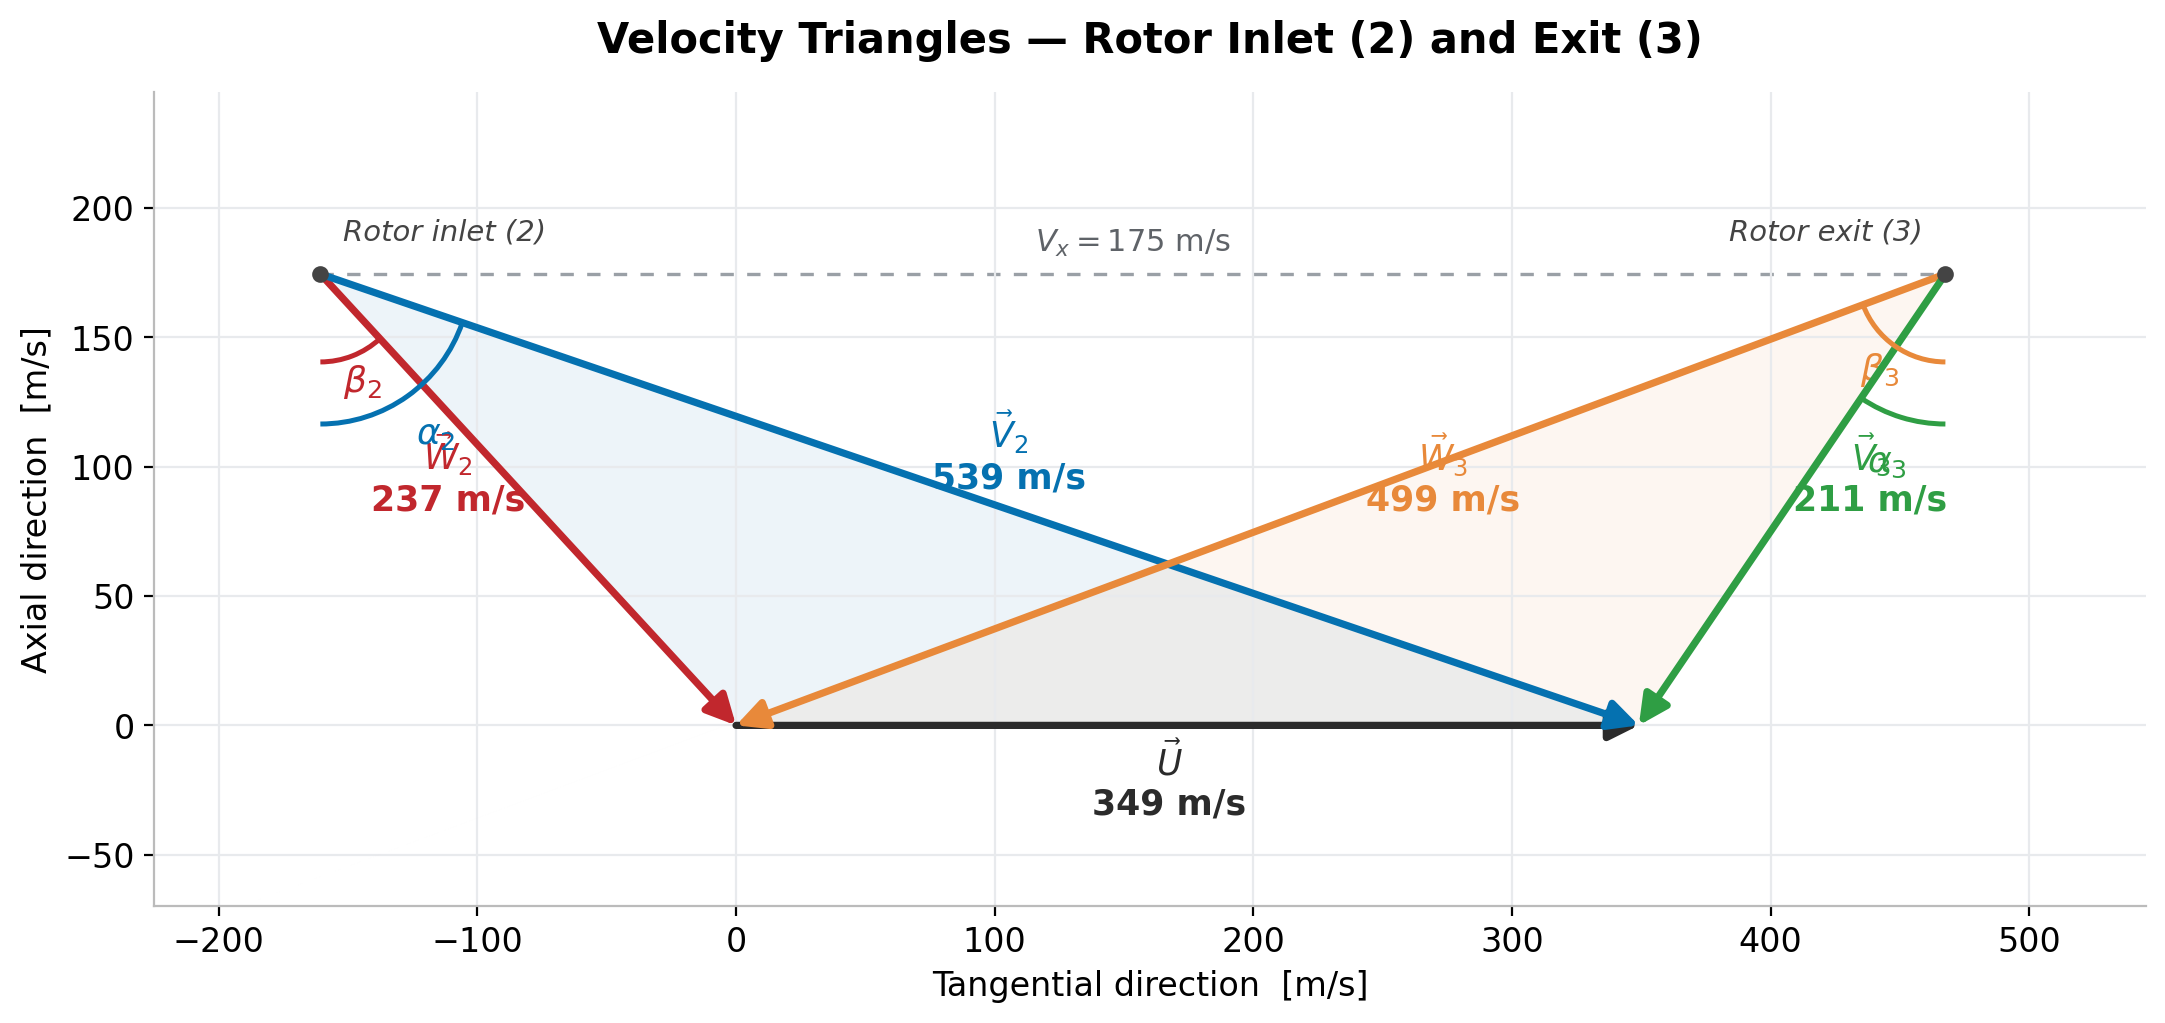
\includegraphics[width=0.8\textwidth]{Velocity Triangles at Rotor Inlet (2) and Exit (3).png}
\caption{Velocity triangles at rotor inlet (station 2) and exit (station 3).}
\label{fig:tri}
\end{figure}

\begin{table}[H]
\centering
\caption{Velocity-triangle parameters.}
\label{tab:tri}
\begin{tabular}{l r r}
\toprule
\textbf{Parameter} & \textbf{Station 2} & \textbf{Station 3}\\
\midrule
$U$ -- blade speed [m/s]        & 349.03 & 349.03 \\
$V$ -- absolute velocity [m/s]  & 538.78 & 210.95 \\
$W$ -- relative velocity [m/s]  & 237.24 & 499.05 \\
$\alpha$ -- flow angle [\degr]  & 71.10  & 34.18 \\
$\beta$ -- blade angle [\degr]  & 42.64  & 69.53 \\
\bottomrule
\end{tabular}
\end{table}

The total turning of the rotor is $\Delta\beta = \beta_2+\beta_3 = 112.2\degr$,
typical of a heavily loaded high-pressure rotor.

% =====================================================================
\section{h--s Diagram}

The enthalpy--entropy diagram (Fig.~\ref{fig:hs}) summarises the expansion: the
isentropic, static and stagnation enthalpies at each station and the kinetic
energy terms $V^2/2$ and $W^2/2$. The enthalpy ladder is listed in
Table~\ref{tab:hs}.

\begin{table}[H]
\centering
\caption{Enthalpy ladder of the stage (J/kg).}
\label{tab:hs}
\begin{tabular}{l r l r}
\toprule
\textbf{Quantity} & \textbf{Value} & \textbf{Quantity} & \textbf{Value}\\
\midrule
$H_{01}=H_{02}$ & 1942338 & $h_3$    & 1700813 \\
$h_1$           & 1935154 & $h_{3s}$ & 1686977 \\
$h_2$           & 1797198 & $h_{3ss}$& 1665655 \\
$h_{2s}$        & 1781071 & $H_{03}$ & 1723063 \\
$H_{0R}$        & 1825338 & $H_{03ss}$& 1687906 \\
\bottomrule
\end{tabular}
\end{table}

\begin{figure}[H]
\centering
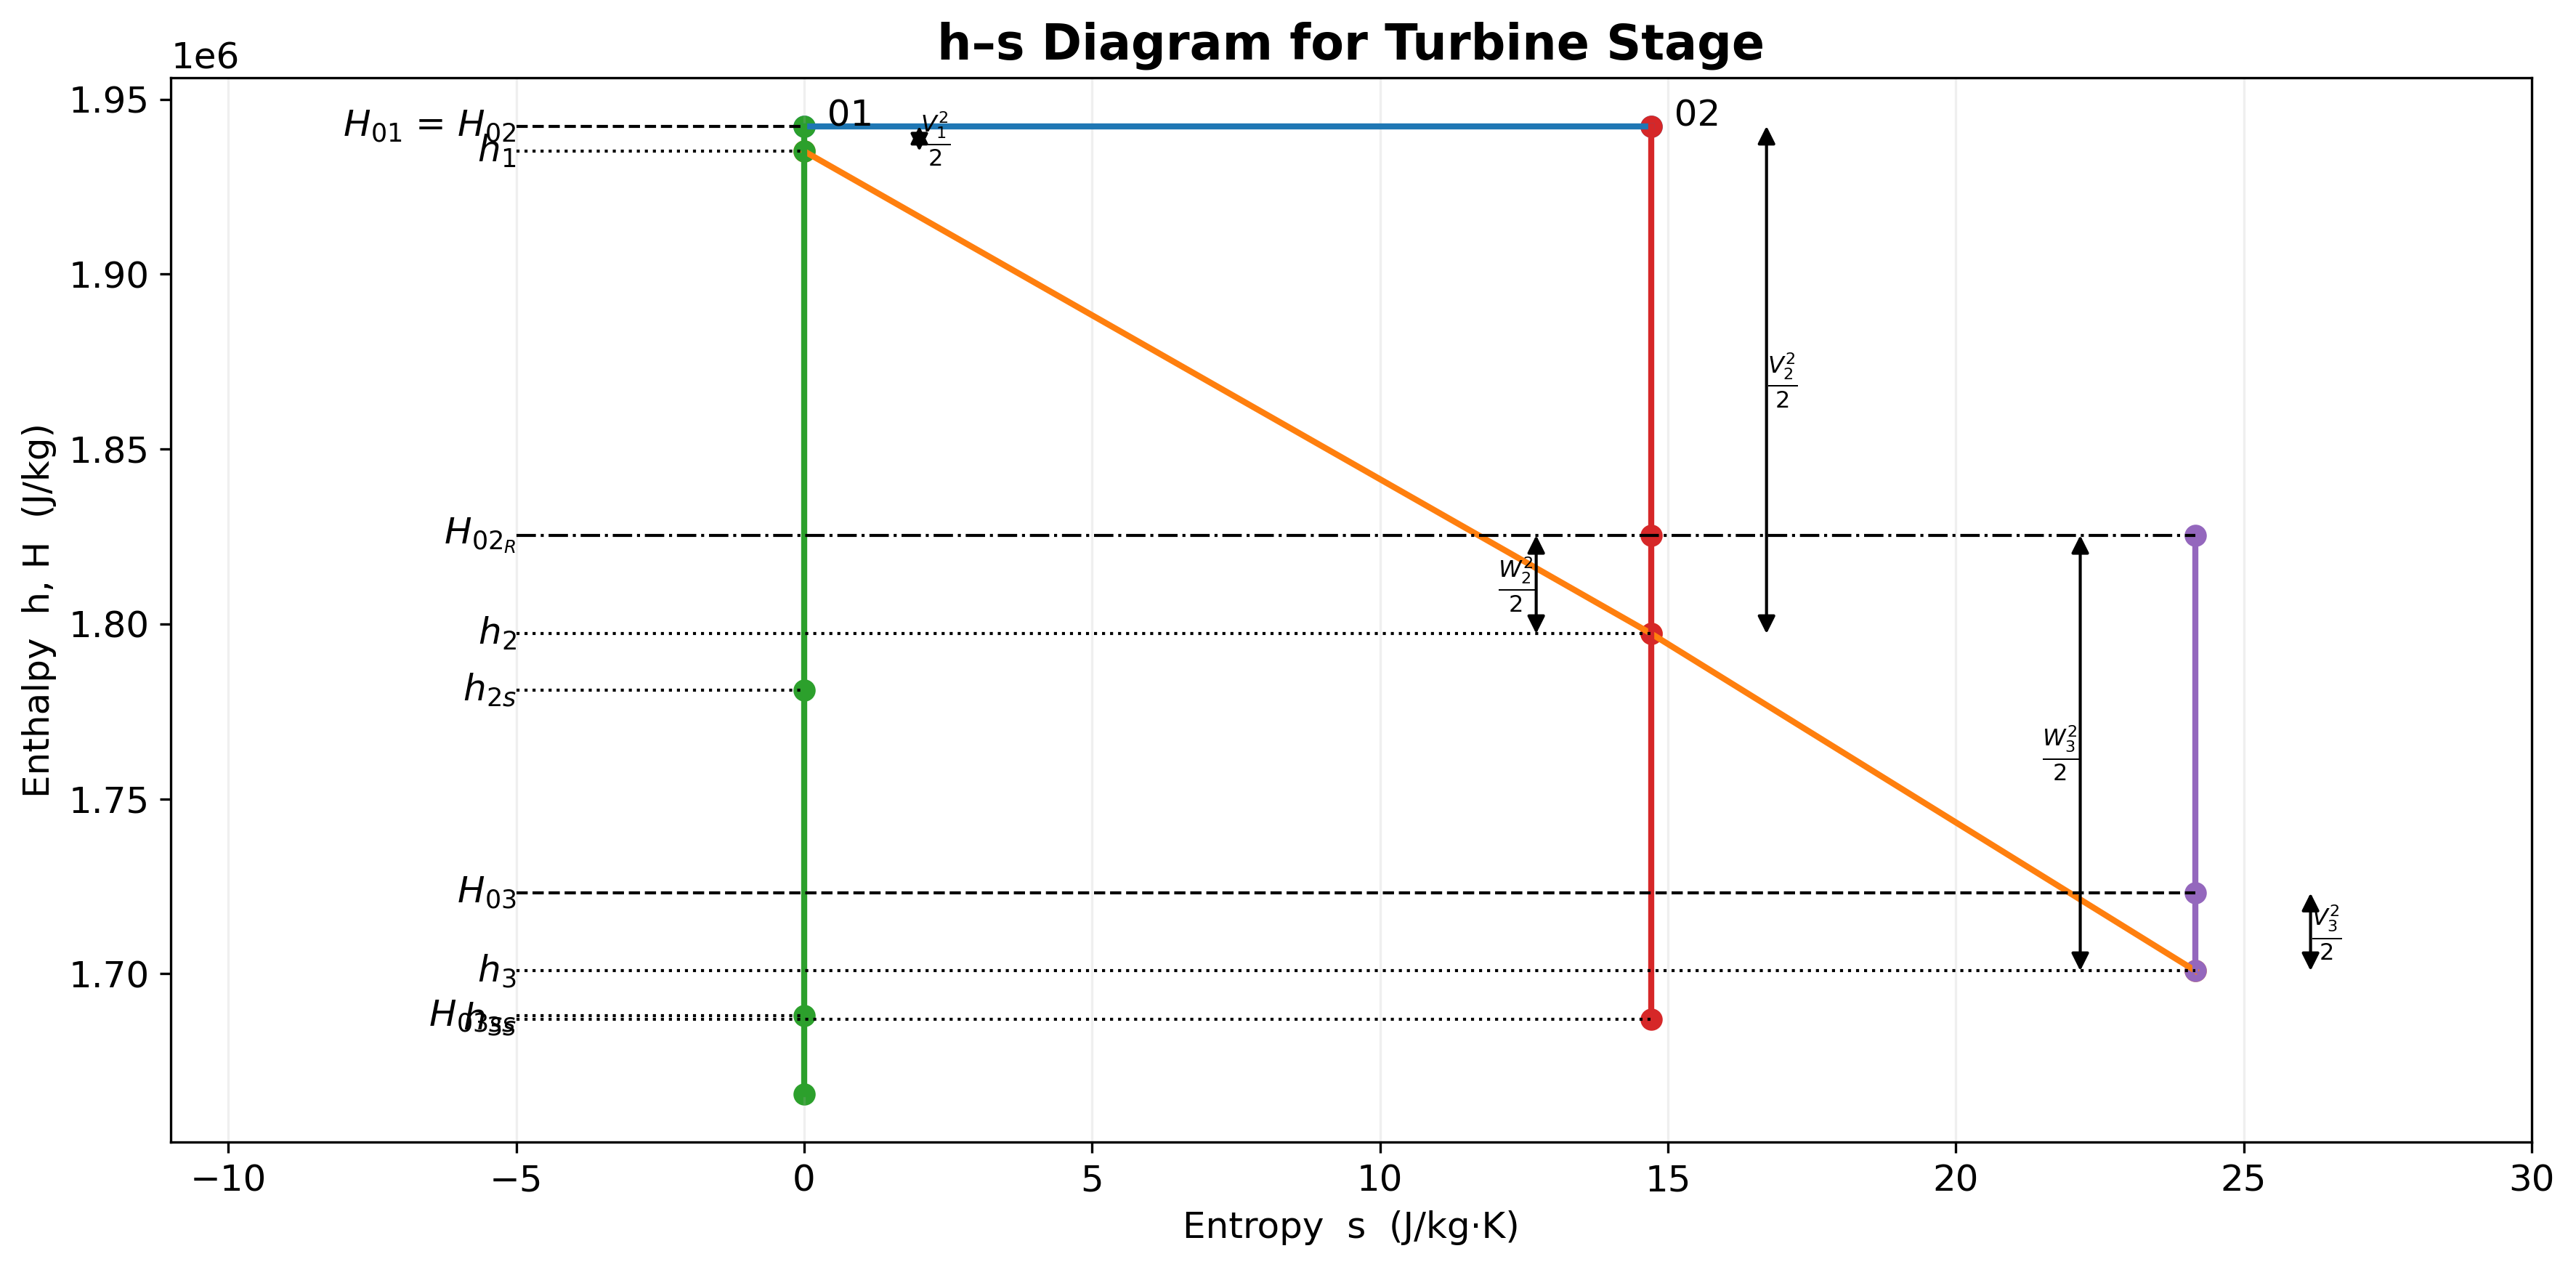
\includegraphics[width=0.9\textwidth]{h-s Diagram for Turbine Stage.png}
\caption{h--s diagram of the first turbine stage.}
\label{fig:hs}
\end{figure}

\subsection{Comparison of Enthalpy (closure of the design)}
\label{sec:enth}

The exit static pressure $P_3$ is not known a priori. The stage enthalpy drop
computed kinematically from the velocity triangles, $\Delta H_0 = c_p(T_{01}-T_{03})$,
must equal the value $\Delta H_{real}=P_{stage}/\dot m$ imposed by the power
balance. A Newton--Raphson loop adjusts $P_3$ until the two agree:
\[
\Delta H_0 < \Delta H_{real} \Rightarrow P_3' < P_3,\quad
\Delta H_0 > \Delta H_{real} \Rightarrow P_3' > P_3,\quad
\Delta H_0 = \Delta H_{real} \Rightarrow \text{OK}.
\]
The loop converges in 33 iterations to
$P_3 = \SI{1107265}{Pa}$, with $\Delta H_0 = \Delta H_{real} = \SI{219.27}{kJ/kg}$
(residual $< \SI{1e-5}{kJ/kg}$).

% =====================================================================
\section{Annulus Sizing}

Annulus sizing fixes the radial extent of the blade row. With a shrouded
end-wall assumption (equal hub and tip contour angles $\varepsilon$), the areas
follow from mass conservation, $A = \dot m/(\rho V_x)$, and the heights from
$h = A/(\pi D_m)$. The mean radius is set by the blade speed,
$R_m = 60\,U_m/(2\pi N) = \SI{1.11}{m}$. Table~\ref{tab:annulus} lists the
results.

\begin{table}[H]
\centering
\caption{Annulus geometry (constant mean radius).}
\label{tab:annulus}
\begin{tabular}{l r}
\toprule
\textbf{Quantity} & \textbf{Value}\\
\midrule
Mean radius $R_m$ [m]            & 1.110 \\
Span $h_2$ [mm]                  & 192.1 \\
Span $h_3$ [mm]                  & 234.6 \\
Tip radius (st.\ 3) $R_{T3}$ [m] & 1.228 \\
Hub radius (st.\ 3) $R_{H3}$ [m] & 0.994 \\
End-wall flare $\varepsilon$ [\degr] & 15.90 \\
$AN^2$ [m$^2$\,rpm$^2$]          & $1.341\times10^{7}$ \\
\bottomrule
\end{tabular}
\end{table}

The end-wall flare angle, obtained from the span growth over the axial chord,
$\varepsilon = \tan^{-1}\!\big((h_3-h_2)/c_x\big) = 15.90\degr$, stays below the
$15$--$20\degr$ range that bounds end-wall separation.

% =====================================================================
\section{Design Constraints}

Table~\ref{tab:constr} compares the obtained values against the aerodynamic and
mechanical design guidelines. Eight of the ten constraints are satisfied; two are
marginally violated -- the stator-exit Mach number $M_2 = 0.700$ sits exactly at
the lower edge of the $0.7$--$0.85$ band, and the span ratio $h_3/h_2 = 1.221$
slightly exceeds the recommended $1.2$. Both are borderline and could be cleared
by a small change of $\psi$, $\phi$ or $r$.

\begin{table}[H]
\centering
\caption{Comparison of design control parameters and obtained results.}
\label{tab:constr}
\begin{tabular}{l c c c}
\toprule
\textbf{Constraint} & \textbf{Design range} & \textbf{Obtained} & \textbf{Status}\\
\midrule
$M_2$              & $0.7$--$0.85$ & 0.700  & FAIL (low) \\
$\beta_2$ [\degr]  & $<47.5$       & 42.64  & PASS \\
$M_{w2}$           & $<0.5$        & 0.308  & PASS \\
$M_{w3}$           & $0.65$--$0.8$ & 0.666  & PASS \\
$\beta_3$ [\degr]  & $<75$         & 69.53  & PASS \\
$\Delta\beta$ [\degr] & $110$--$120$ & 112.17 & PASS \\
$M_3$              & $0.3$         & 0.300  & PASS \\
$\alpha_3$ [\degr] & $<35$         & 34.18  & PASS \\
$h_3/h_2$          & $<1.2$        & 1.221  & FAIL (high) \\
$AN^2$ [m$^2$rpm$^2$] & $<3\times10^7$ & $1.34\times10^7$ & PASS \\
\bottomrule
\end{tabular}
\end{table}

% ------------------------------- Chapter 3 -------------------------------
\chapter{Rotor Blade Design}

The rotor-blade design converts the mean-line flow angles into an actual blade
profile. A few geometric assumptions (aspect ratio, stagger) fix the chord and
the number of blades, after which the camber line and the thickness distribution
are built with ParaBlade from the inlet/exit metal angles.

% =====================================================================
\section{Input Data Assumptions}

\paragraph{Aspect ratio $AR = b/\bar c$.}
The aspect ratio relates the blade span $b$ to the chord $\bar c$. For
high-pressure rotors $AR$ lies between $1$ and $1.5$; a value $AR = 1$ is adopted,
which gives the best compromise for the present loading.

\paragraph{Stagger angle $\xi$.}
The stagger is the angle between the chord and the axial direction. It is read
from the Kacker \& Okapuu correlation~\cite{kacker} as a function of the inlet and
exit relative angles $\beta_2 = 42.64\degr$ and $\beta_3 = 69.53\degr$, giving
$\xi \approx 39\degr$.

\paragraph{Zweifel loading coefficient.}
The blade pitch (and hence the blade count) is set from the Zweifel
criterion~\cite{zweifel} with $Z = 1.0$, which fixes the optimum
pitch-to-axial-chord ratio for the prescribed turning.

% =====================================================================
\section{Design Procedure and Calculations}

From the aspect ratio and the span, the chord and axial chord are obtained; the
Zweifel criterion then fixes the pitch and, with the mean circumference, the
number of blades:
\begin{equation}
    N_b = \frac{2\pi R_m}{s},\qquad s = \text{pitch}.
\end{equation}
The camber line is generated between the metal angles $\beta_2$ (inlet) and
$\beta_3$ (exit) and combined with a prescribed thickness distribution to produce
the suction and pressure surfaces using ParaBlade~\cite{parablade}. The tool
reproduces the prescribed analytic curvature: a check of the curvature design
variable against the analytic surface curvature matches at both ends
($\kappa_{LE}=17.61$, $\kappa_{TE}=213.29$), confirming a consistent profile.

% =====================================================================
\section{Main Blade Parameters}

The resulting blade parameters are collected in Table~\ref{tab:blade}; the
constructed section is shown in Fig.~\ref{fig:section}.





\begin{minipage}{0.58\textwidth}
    \begin{table}[H]
\centering
\caption{Main rotor-blade parameters.}
\label{tab:blade}
\begin{tabular}{l r}
\toprule
\textbf{Parameter} & \textbf{Value}\\
\midrule
Inlet flow angle $\alpha_2$ [\degr]          & 71.10 \\
Inlet metal (rel.) angle $\beta_2$ [\degr]   & 42.64 \\
Exit flow angle $\alpha_3$ [\degr]           & 34.18 \\
Exit metal (rel.) angle $\beta_3$ [\degr]    & 69.53 \\
Aspect ratio $AR$                            & 1.00 \\
Stagger angle $\xi$ [\degr]                   & 39.0 \\
Zweifel coefficient $Z$                      & 1.00 \\
Chord $c$ [m]                                & 0.192 \\
Axial chord $c_x$ [m]                        & 0.149 \\
Pitch $s$ [m]                                & 0.170 \\
Pitch-to-axial-chord $s/c_x$                 & 1.14 \\
Number of blades $N_b$                       & 42 \\
Max. thickness-to-chord $t_{max}/c$          & 0.20 \\
Leading-edge radius $R_{LE}$ [m]             & 0.0085 \\
Trailing-edge radius $R_{TE}$ [m]            & 0.0007 \\
End-wall flare angle $\varepsilon$ [\degr]    & 15.90 \\
\bottomrule
\end{tabular}
\end{table}
\end{minipage}
\hfill
\begin{minipage}{0.38\textwidth}
    \begin{figure}[H]
\centering
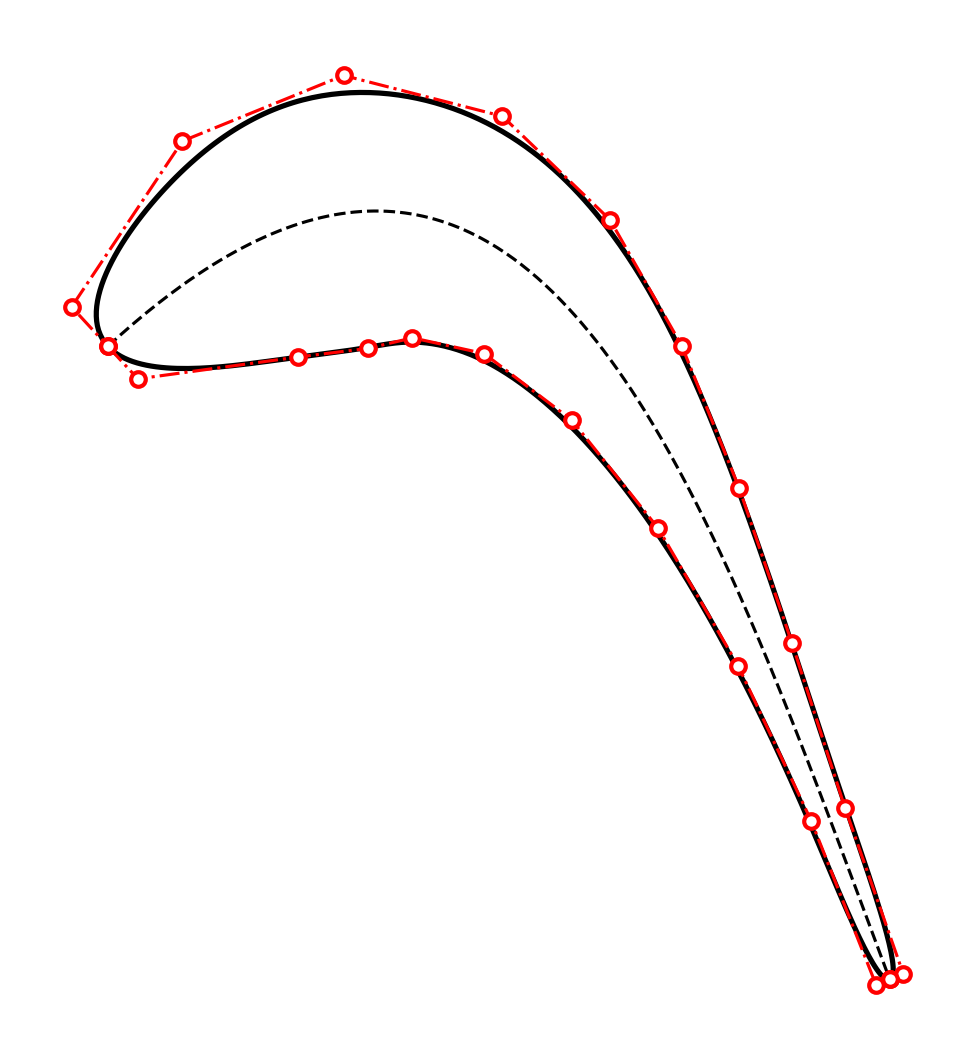
\includegraphics[width=0.55\textwidth]{Blade Section.png}
\caption{Constructed rotor-blade section (camber line and thickness distribution).}
\label{fig:section}
\end{figure}
\end{minipage}
% ------------------------------- Chapter 4 -------------------------------
\chapter{Rotor Blade Construction and CFD Evaluation}

The blade profile obtained in Chapter~3 is assembled into a linear cascade and
evaluated with a 2-D RANS computation. This chapter describes the passage
geometry, the mesh, the solver setup and convergence, and the post-processed
aerodynamic results (loading, Mach/pressure fields and the exit wake).

% =====================================================================
\section{Blade Passage Geometry}

The cascade is modelled as three blades: the central (measured) blade and its two
neighbours, whose facing surfaces form the upper and lower passage walls. The
non-dimensional pitch and throat characterise the passage:
\begin{equation}
    s/c_x = 1.136,\quad o/c_x = 0.805,\quad o/s = 0.709,\quad
    (x/c_x)_{throat} = 0.284,
\end{equation}
with dimensional values $c_x = \SI{0.149}{m}$, $s = \SI{0.170}{m}$ and throat
$o = \SI{0.120}{m}$, for $N_b = 42$ blades.

\section{Evaluation of Profile Curvature and Passage Area}

The prescribed thickness distribution and the analytic curvature of the surfaces
are shown in Fig.~\ref{fig:thkcur}; the passage-width (area) variation along the
axial direction, which contracts monotonically to the throat, is shown in
Fig.~\ref{fig:passwidth}. A smooth, monotonic contraction without local
diffusion is desirable to avoid boundary-layer growth on the suction side.


\begin{figure}[H]
\centering
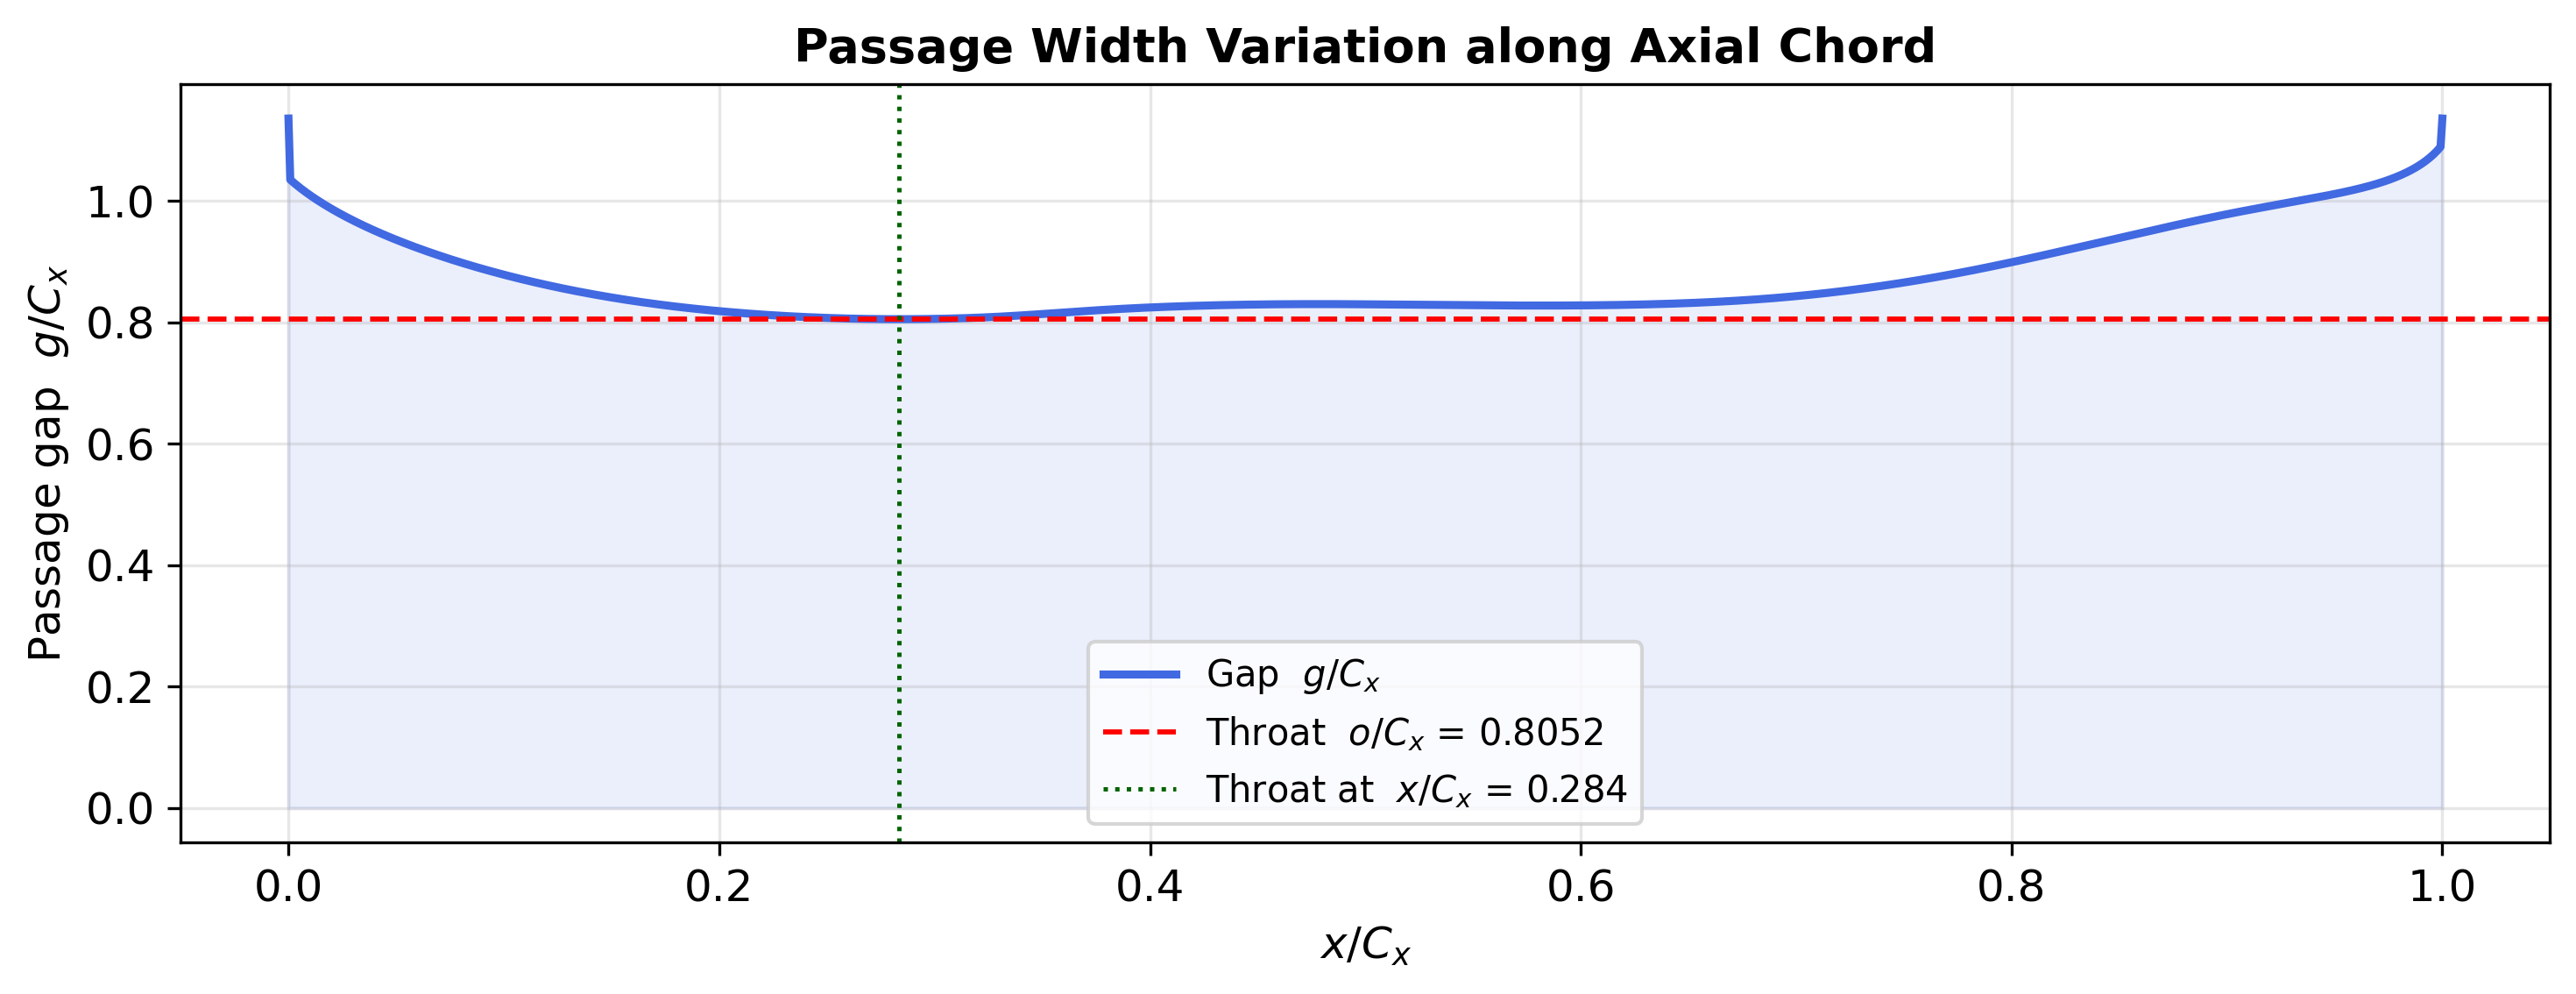
\includegraphics[width=0.7\textwidth]{Passage Width Variation.png}
\caption{Passage-width (area) variation through the blade row.}
\label{fig:passwidth}
\end{figure}

\begin{figure}[H]
\centering
\begin{subfigure}{0.3\textwidth}
    
\includegraphics[width=\textwidth]{Blade Cascade.png}
    \caption{Cascade of rotor blades.}
\end{subfigure}\hfill
\begin{subfigure}{0.4\textwidth}
    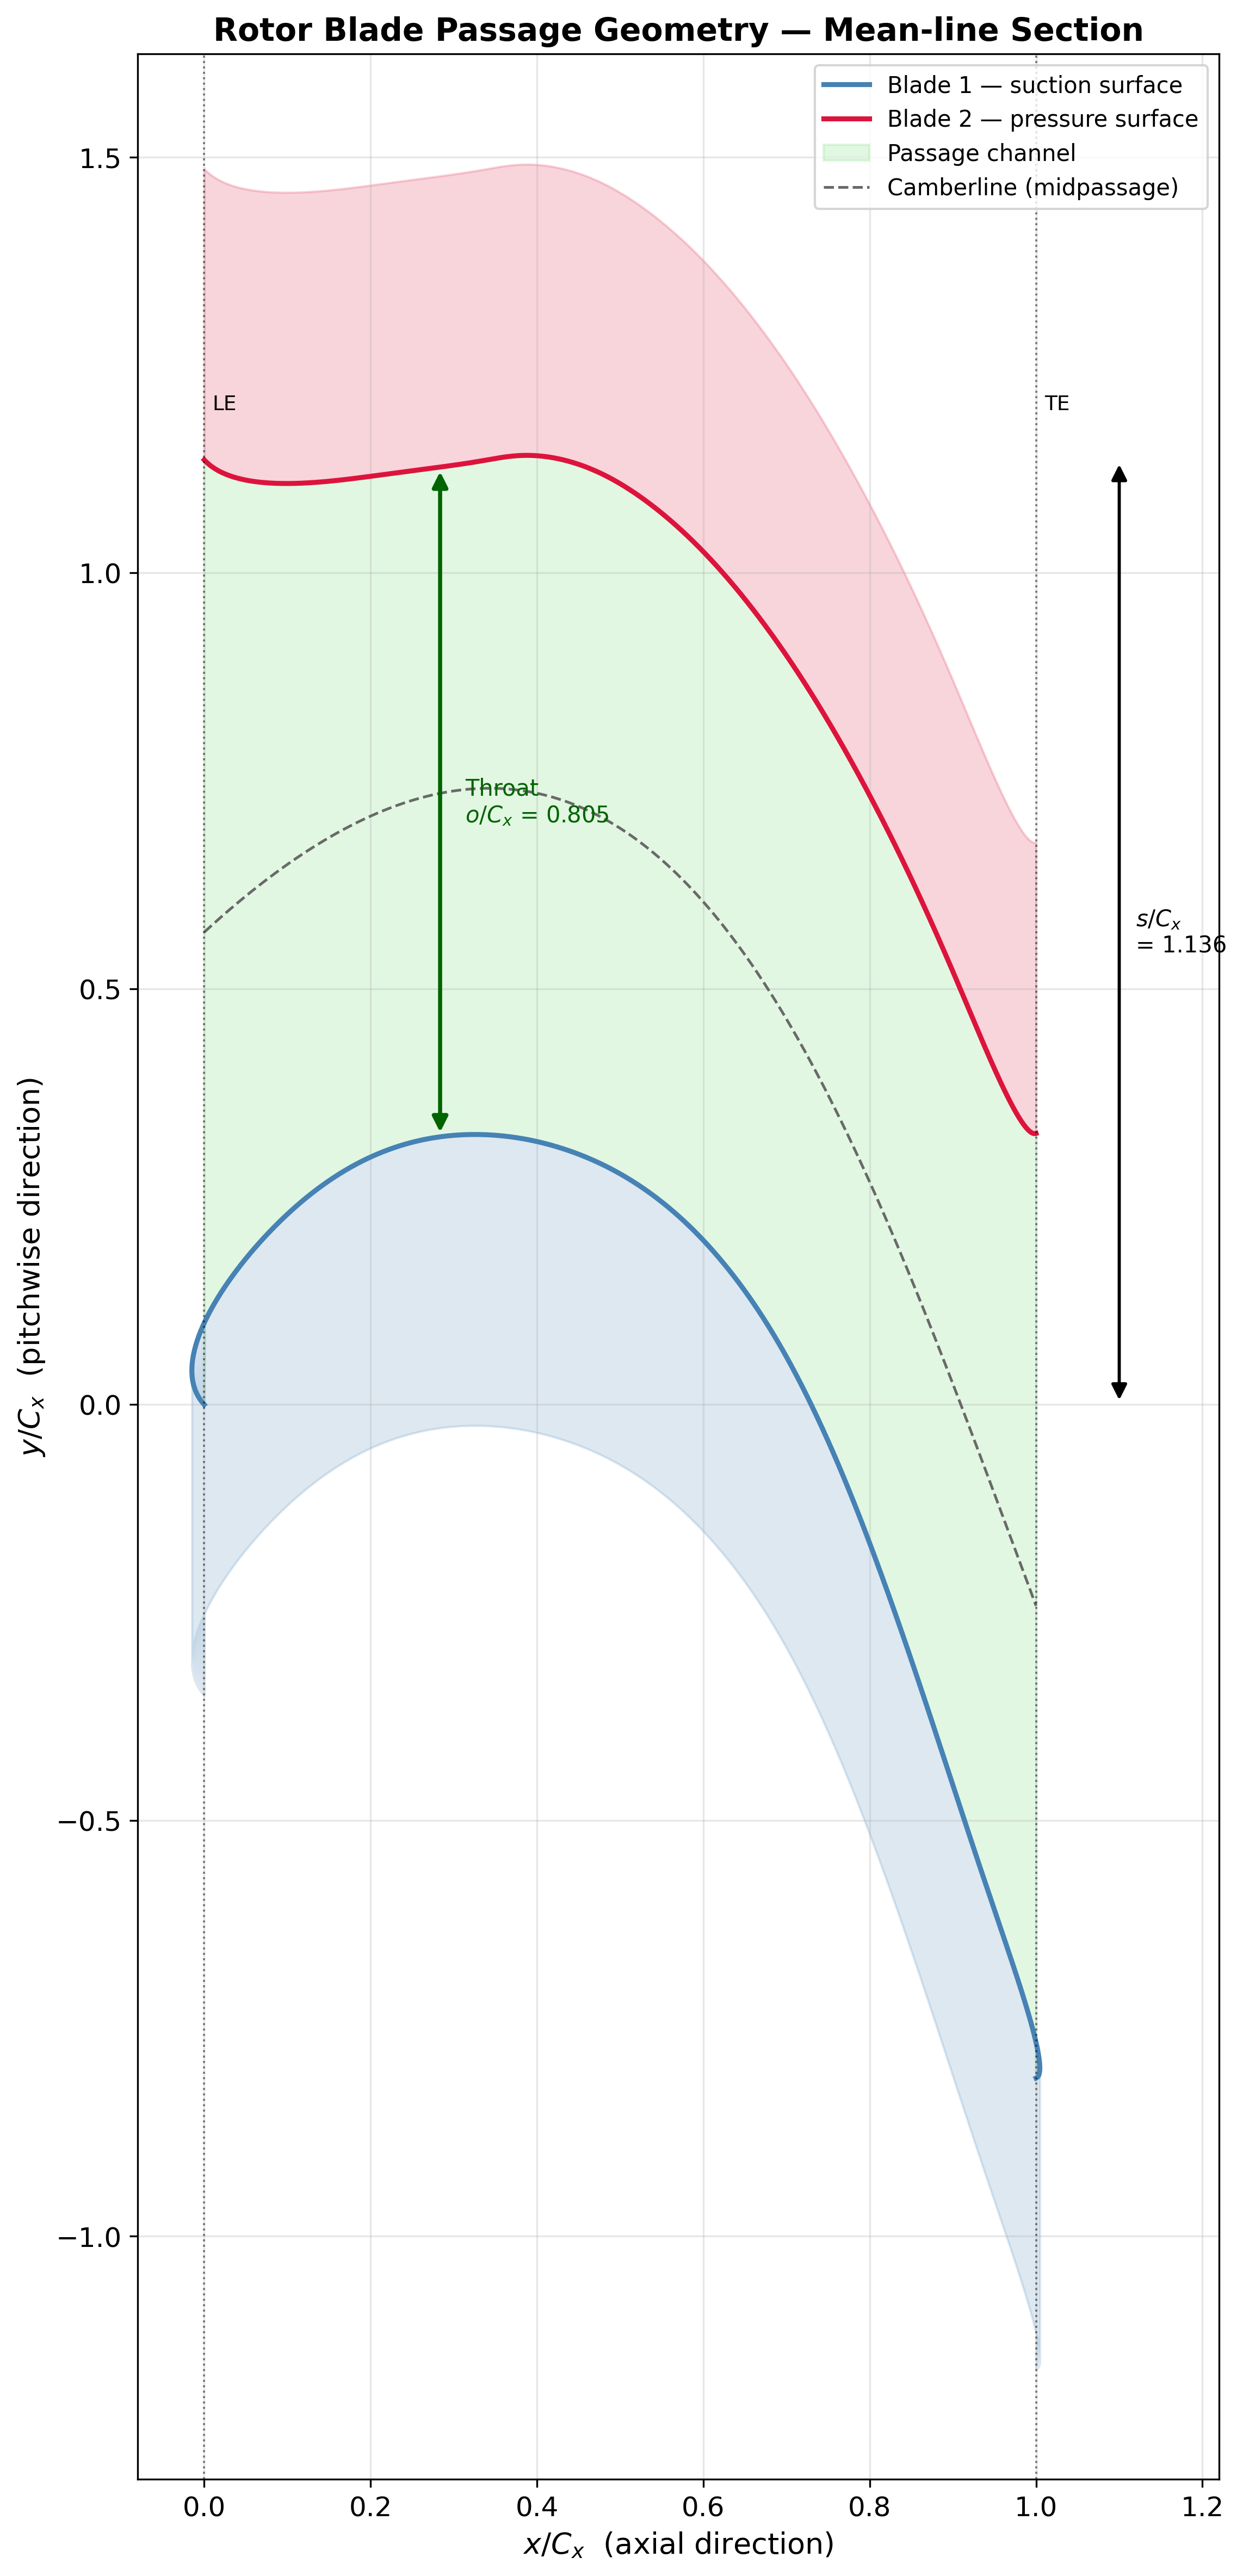
\includegraphics[width=\textwidth]{Rotor Blade Passage Geometry.png}
    \caption{Blade-to-blade passage and throat.}
\end{subfigure}
\caption{Rotor-blade cascade and passage geometry.}
\label{fig:passage}
\end{figure}

% =====================================================================

\begin{figure}[H]
\centering
\begin{subfigure}{0.48\textwidth}
    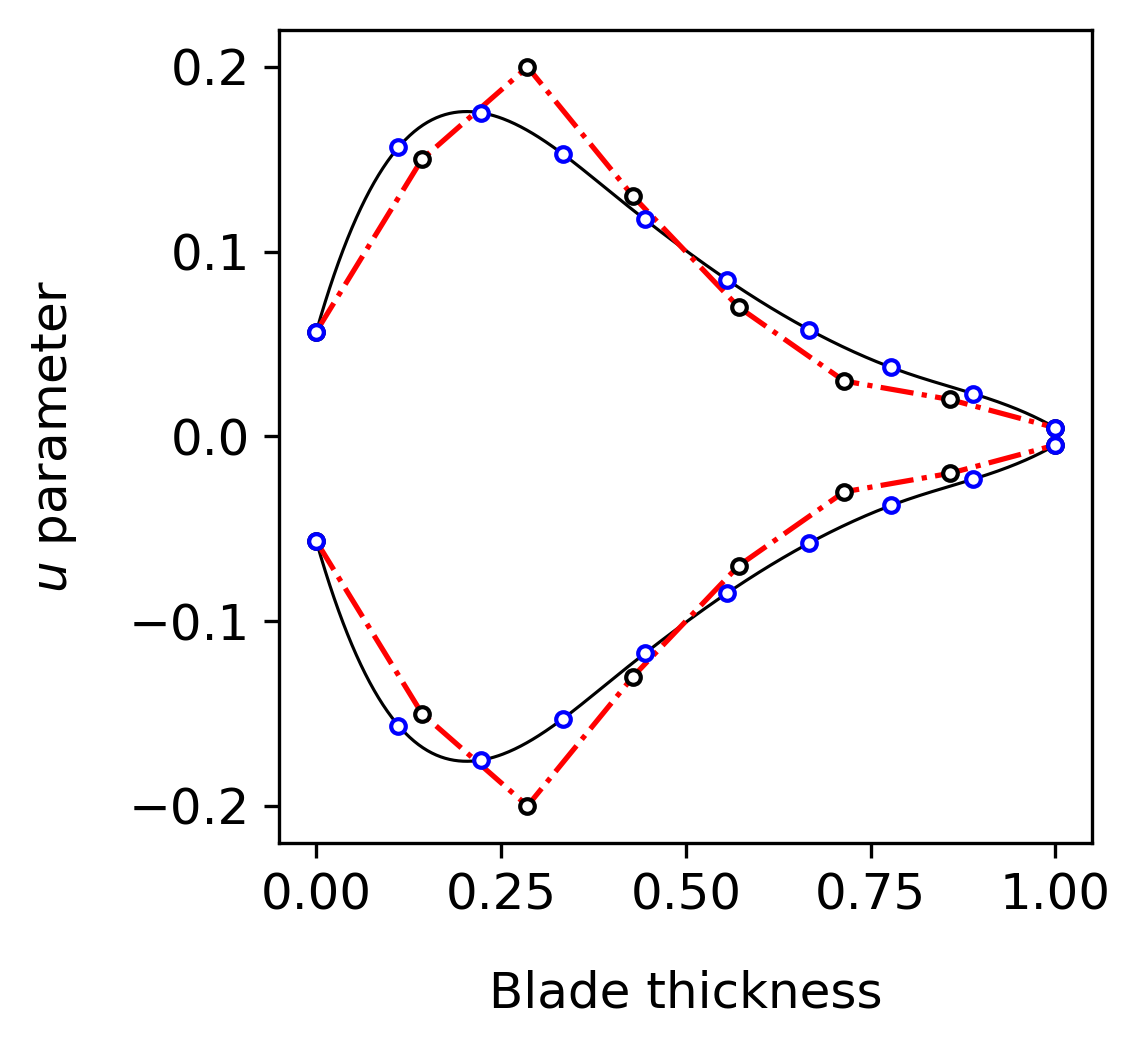
\includegraphics[width=\textwidth]{Thickness Distribution.png}
    \caption{Thickness distribution.}
\end{subfigure}\hfill
\begin{subfigure}{0.48\textwidth}
    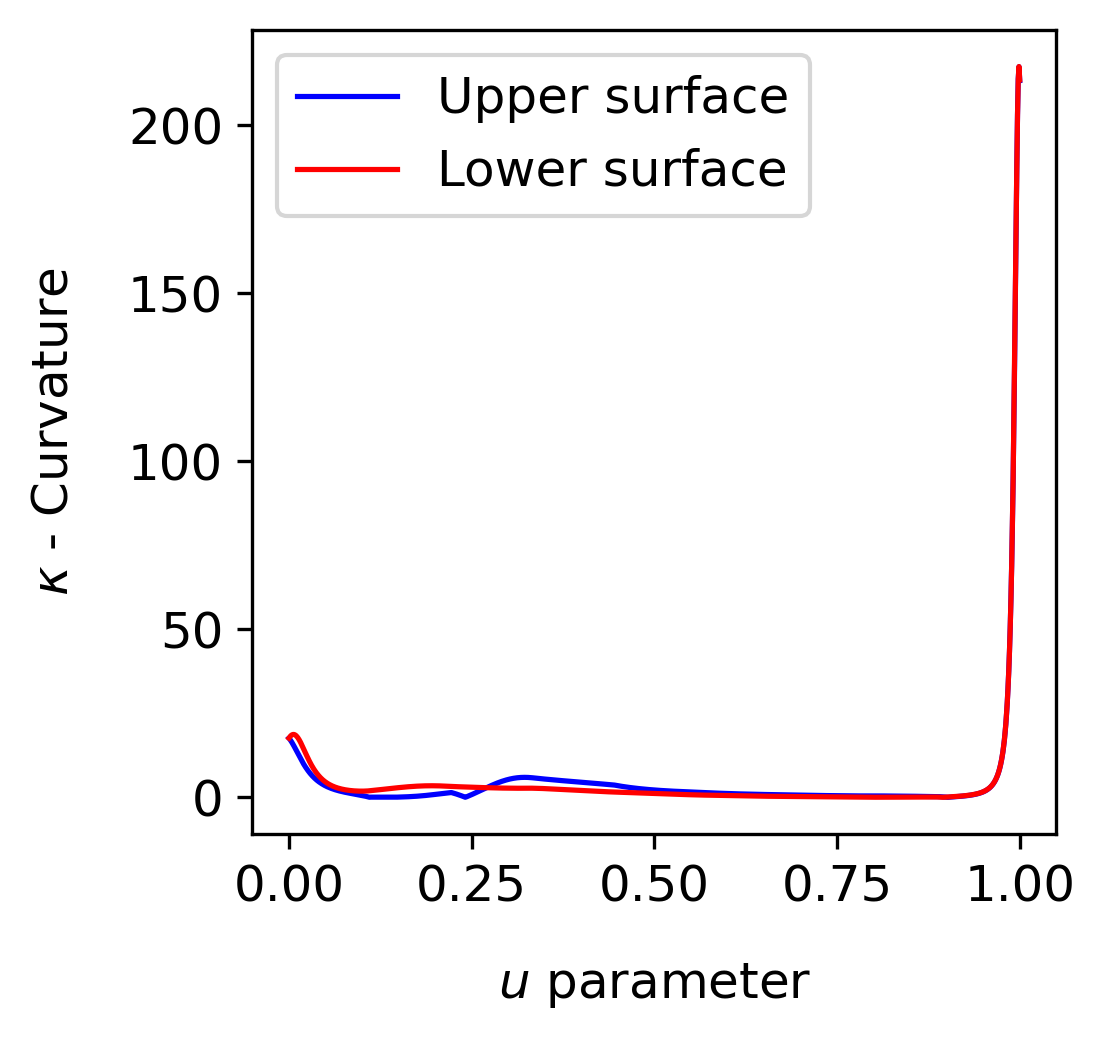
\includegraphics[width=\textwidth]{Curvature Distribution.png}
    \caption{Curvature $\kappa$ distribution.}
\end{subfigure}
\caption{Profile thickness and curvature along the normalised surface coordinate.}
\label{fig:thkcur}
\end{figure}



% =====================================================================
\section{CFD Evaluation}

\subsection{Mesh Generation}

An unstructured triangular mesh is generated with GMSH~\cite{gmsh} over the
three-blade passage. The domain is bounded by the central blade (no-slip wall),
the two neighbour walls (the pressure side of the upper blade and the suction side
of the lower blade), and inlet/outlet planes extended half an axial chord upstream
and downstream along the flow angles $+\beta_2$ and $-\beta_3$. The inlet and
outlet heights are both $\approx 2s = \SI{339.2}{mm}$. A distance-based size field
refines the cells near all blade walls. The mesh contains about $1.81\times10^4$
nodes and $3.54\times10^4$ elements.


\begin{figure}[H]
\centering
\begin{subfigure}{0.35\textwidth}
    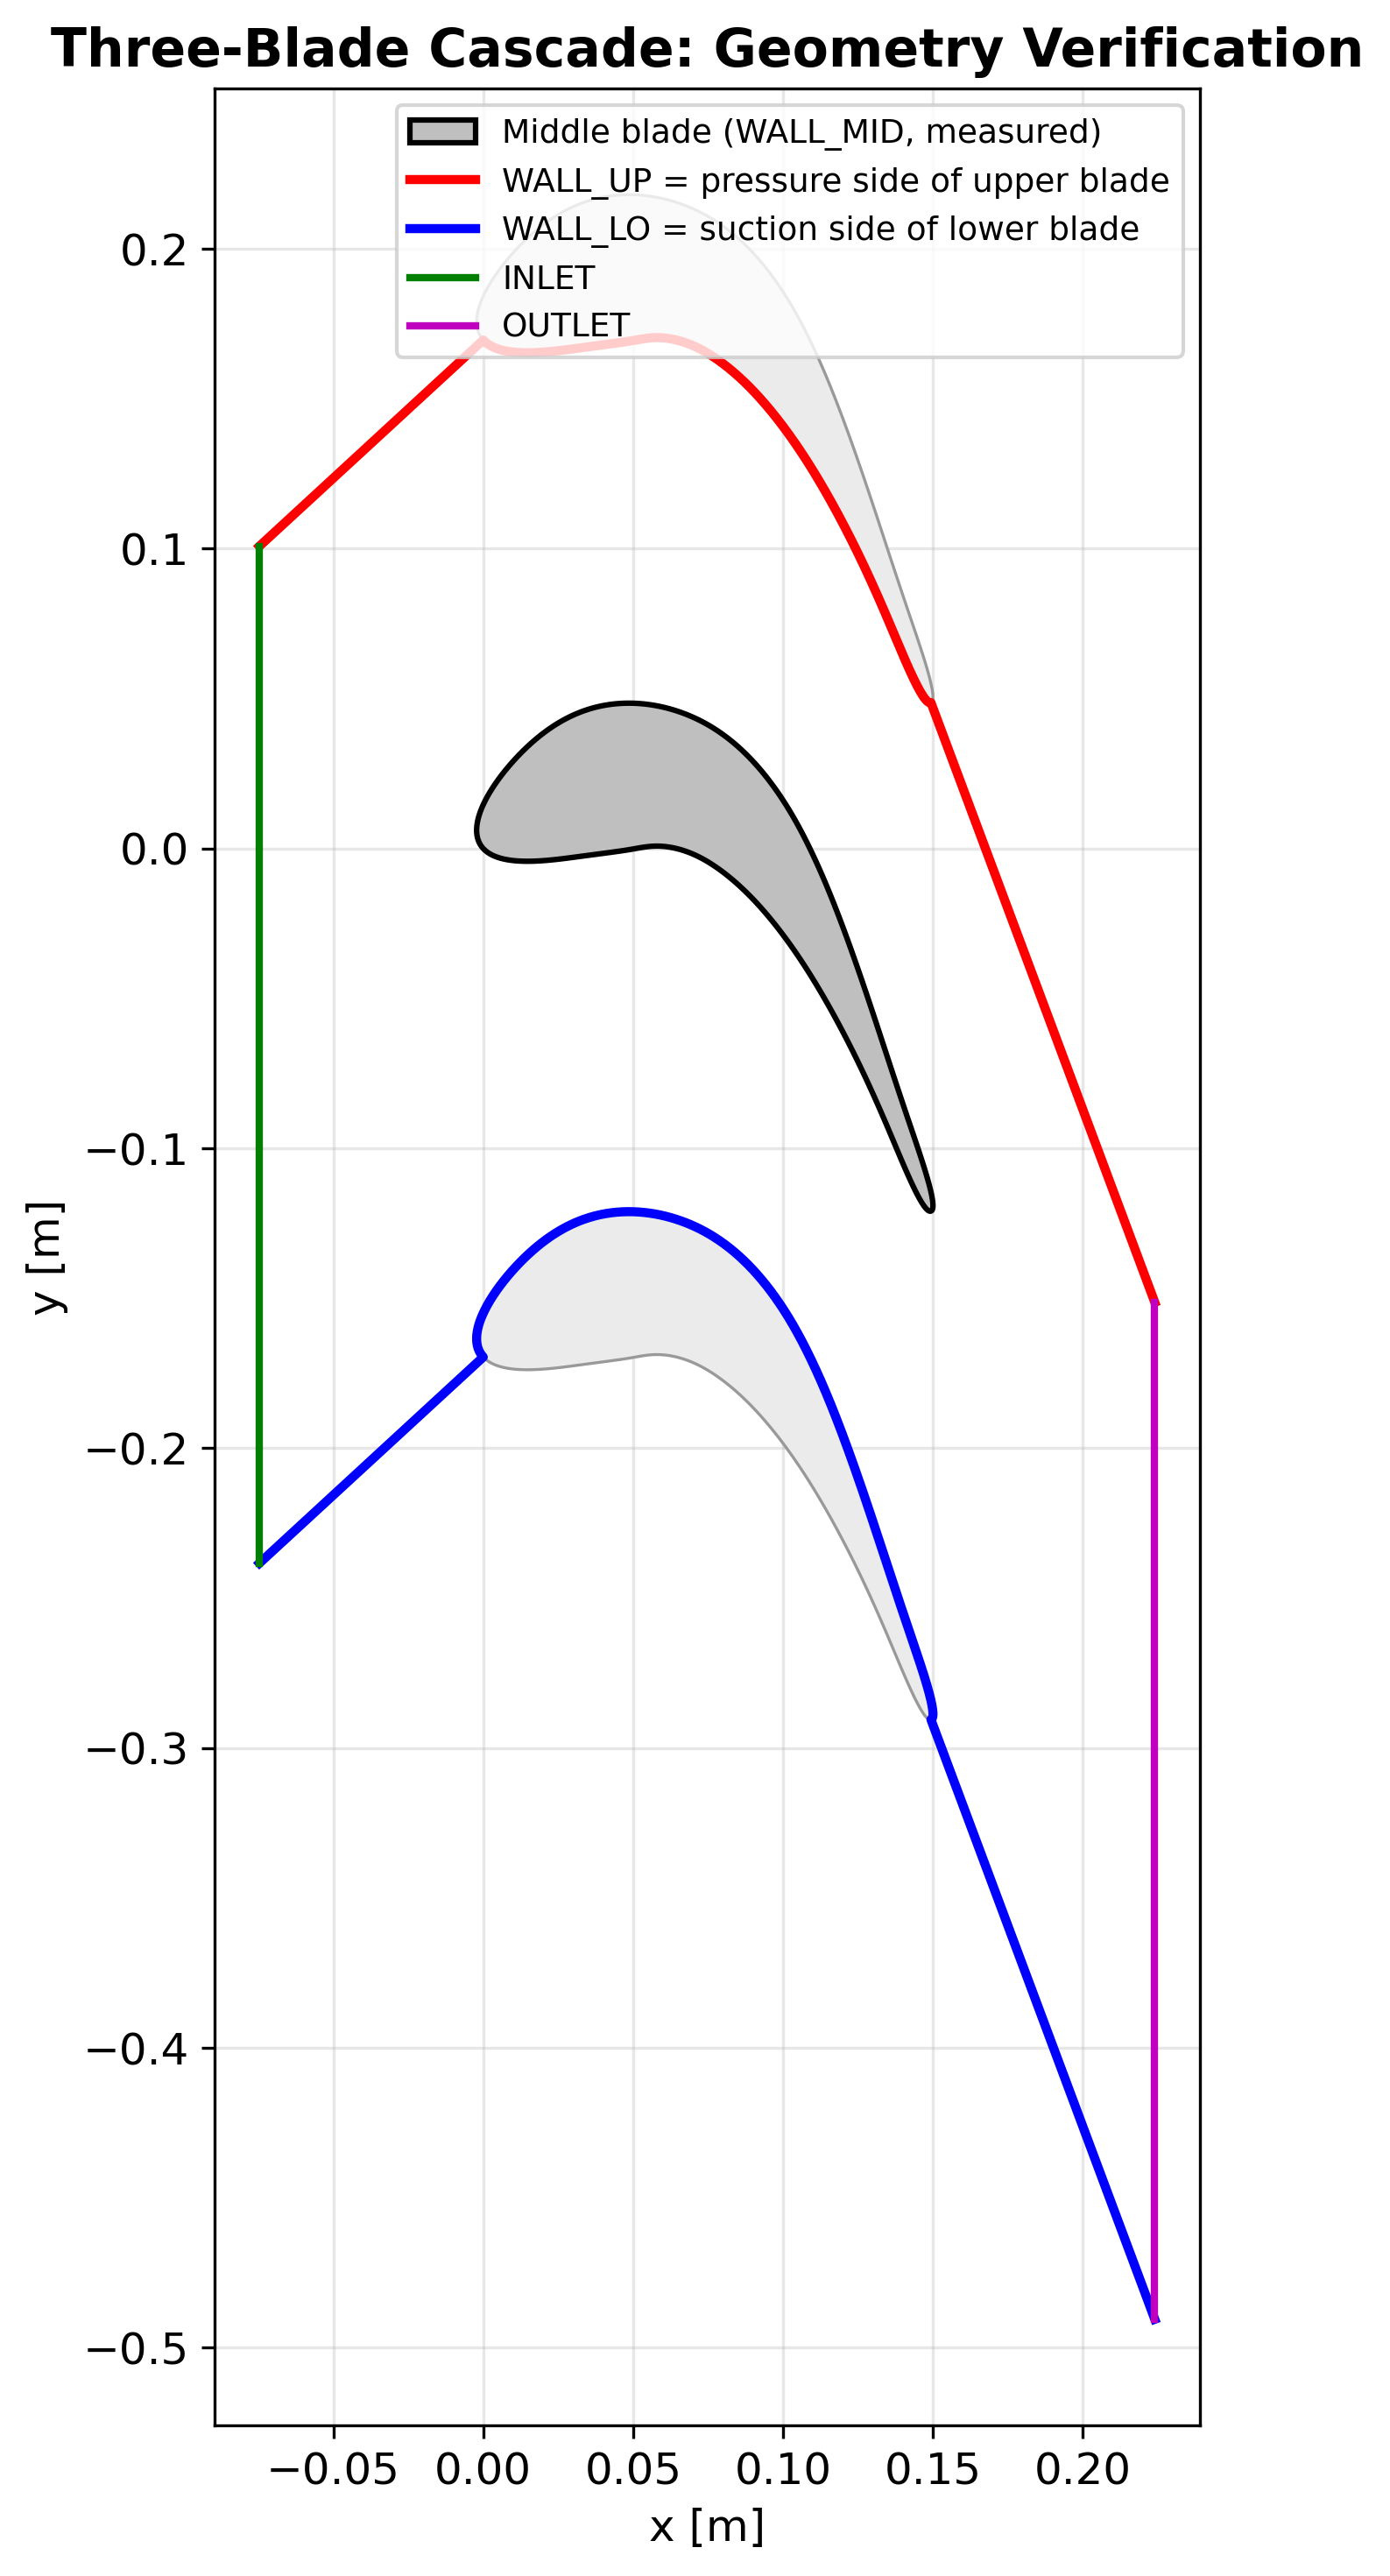
\includegraphics[width=\textwidth]{Mesh-geo-verification.png}
    \caption{Geometry verification of the 3-blade domain.}
\end{subfigure}\hfill
\begin{subfigure}{0.65\textwidth}
    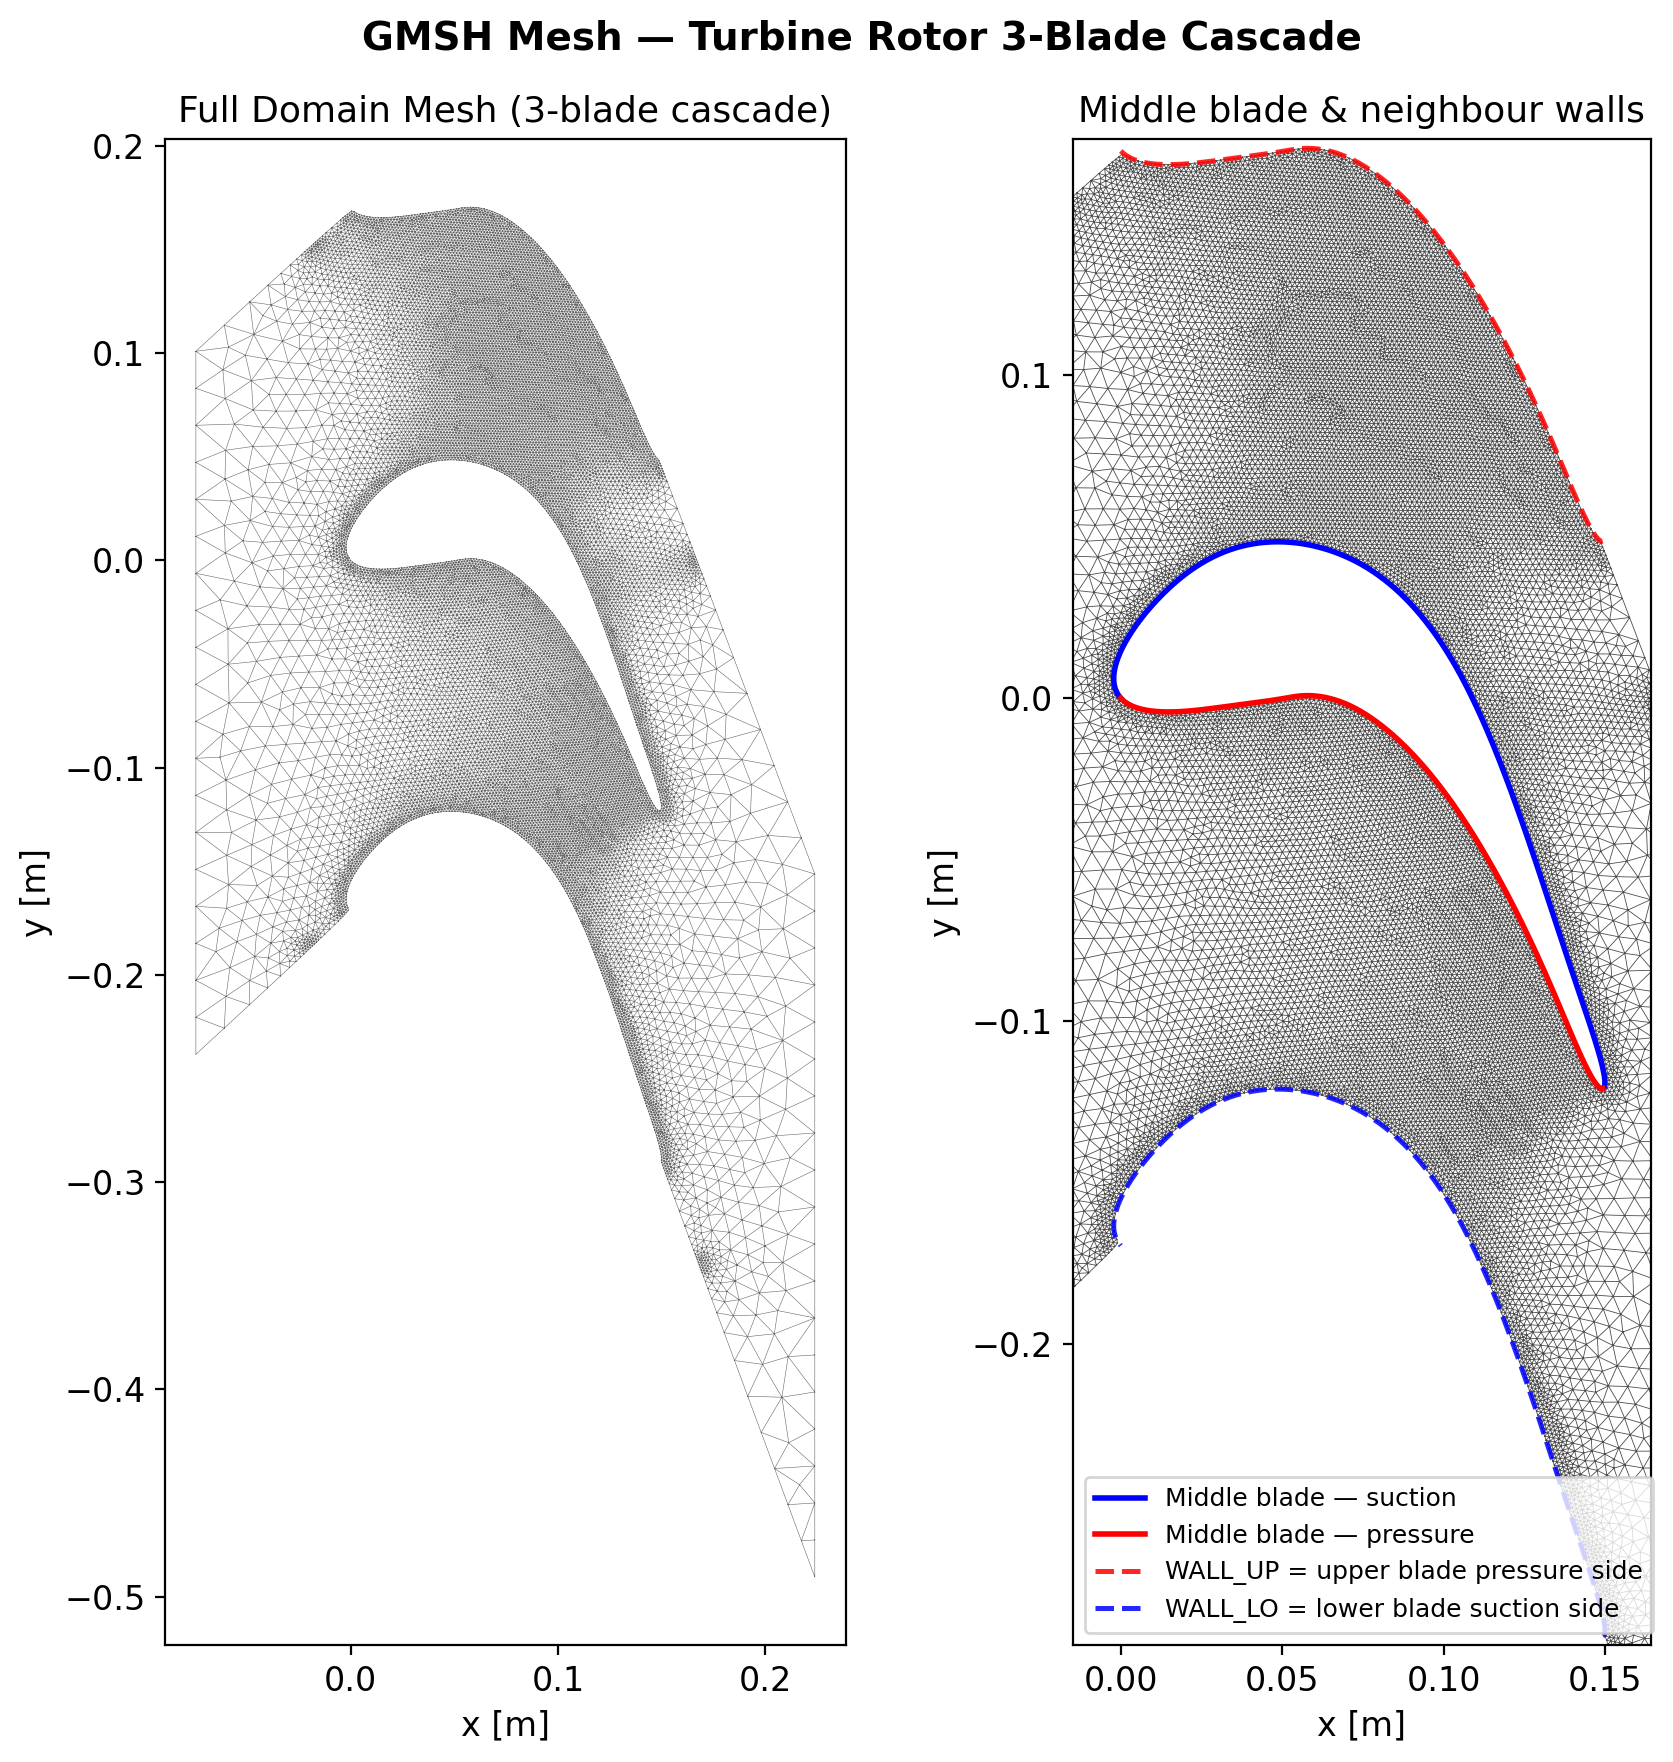
\includegraphics[width=\textwidth]{Blade-mesh.png}
    \caption{Generated GMSH mesh.}
\end{subfigure}
\caption{Three-blade cascade domain and mesh.}
\label{fig:mesh}
\end{figure}


\subsection{CFD Setting}

The flow is solved with SU2~\cite{su2} (compressible RANS, Spalart--Allmaras
turbulence model). The boundary conditions are imposed in the rotor-relative
frame: stagnation inlet from station~2 ($T_{02R}$, $P_{02R}$, flow direction
$\beta_2$), static back-pressure $P_3$ at the outlet, a no-slip adiabatic central
blade and inviscid (Euler) neighbour walls. The main settings are listed in
Table~\ref{tab:su2}.


\begin{table}[H]
\centering
\caption{SU2 CFD solver configuration.}
\label{tab:su2}
\begin{tabular}{l l}
\toprule
\textbf{Setting} & \textbf{Value}\\
\midrule
Solver                       & RANS (compressible) \\
Turbulence model             & Spalart--Allmaras \\
Inlet total temperature $T_{02R}$ [K] & 1578.1 \\
Inlet total pressure $P_{02R}$ [Pa]   & 1521338 \\
Inlet flow angle $\beta_2$ [\degr]    & 42.64 \\
Outlet static pressure $P_3$ [Pa]     & 1107265 \\
Inlet relative Mach $M_{w2}$          & 0.308 \\
Central blade (WALL\_MID)    & no-slip, adiabatic \\
Neighbour walls (WALL\_UP/LO)& Euler (slip) \\
Convergence monitor          & RMS density residual \\
\bottomrule
\end{tabular}
\end{table}

\subsection{CFD Convergence}

The simulation is advanced until the density residual drops by several orders of
magnitude (RMS$[\rho]$ falling below $-7.7$), at which point the surface loading
and the integral exit quantities are stationary. The solution is then used for
the post-processing below.

% =====================================================================
\section{Isentropic Static-Pressure Distribution}

The blade loading is examined through the isentropic Mach number and the static
pressure on the suction and pressure surfaces (Fig.~\ref{fig:loading}). The
suction-side isentropic Mach number rises to $M_{is}\approx 0.84$ near the throat
before recovering, while the pressure side stays below $\approx 0.79$; the static
pressure spans $1.02$--$\SI{1.53}{MPa}$ on the pressure side and
$0.98$--$\SI{1.52}{MPa}$ on the suction side. The loading is front-to-mid loaded
with no sign of suction-side separation.

\begin{figure}[H]
\centering
\begin{subfigure}{0.48\textwidth}
    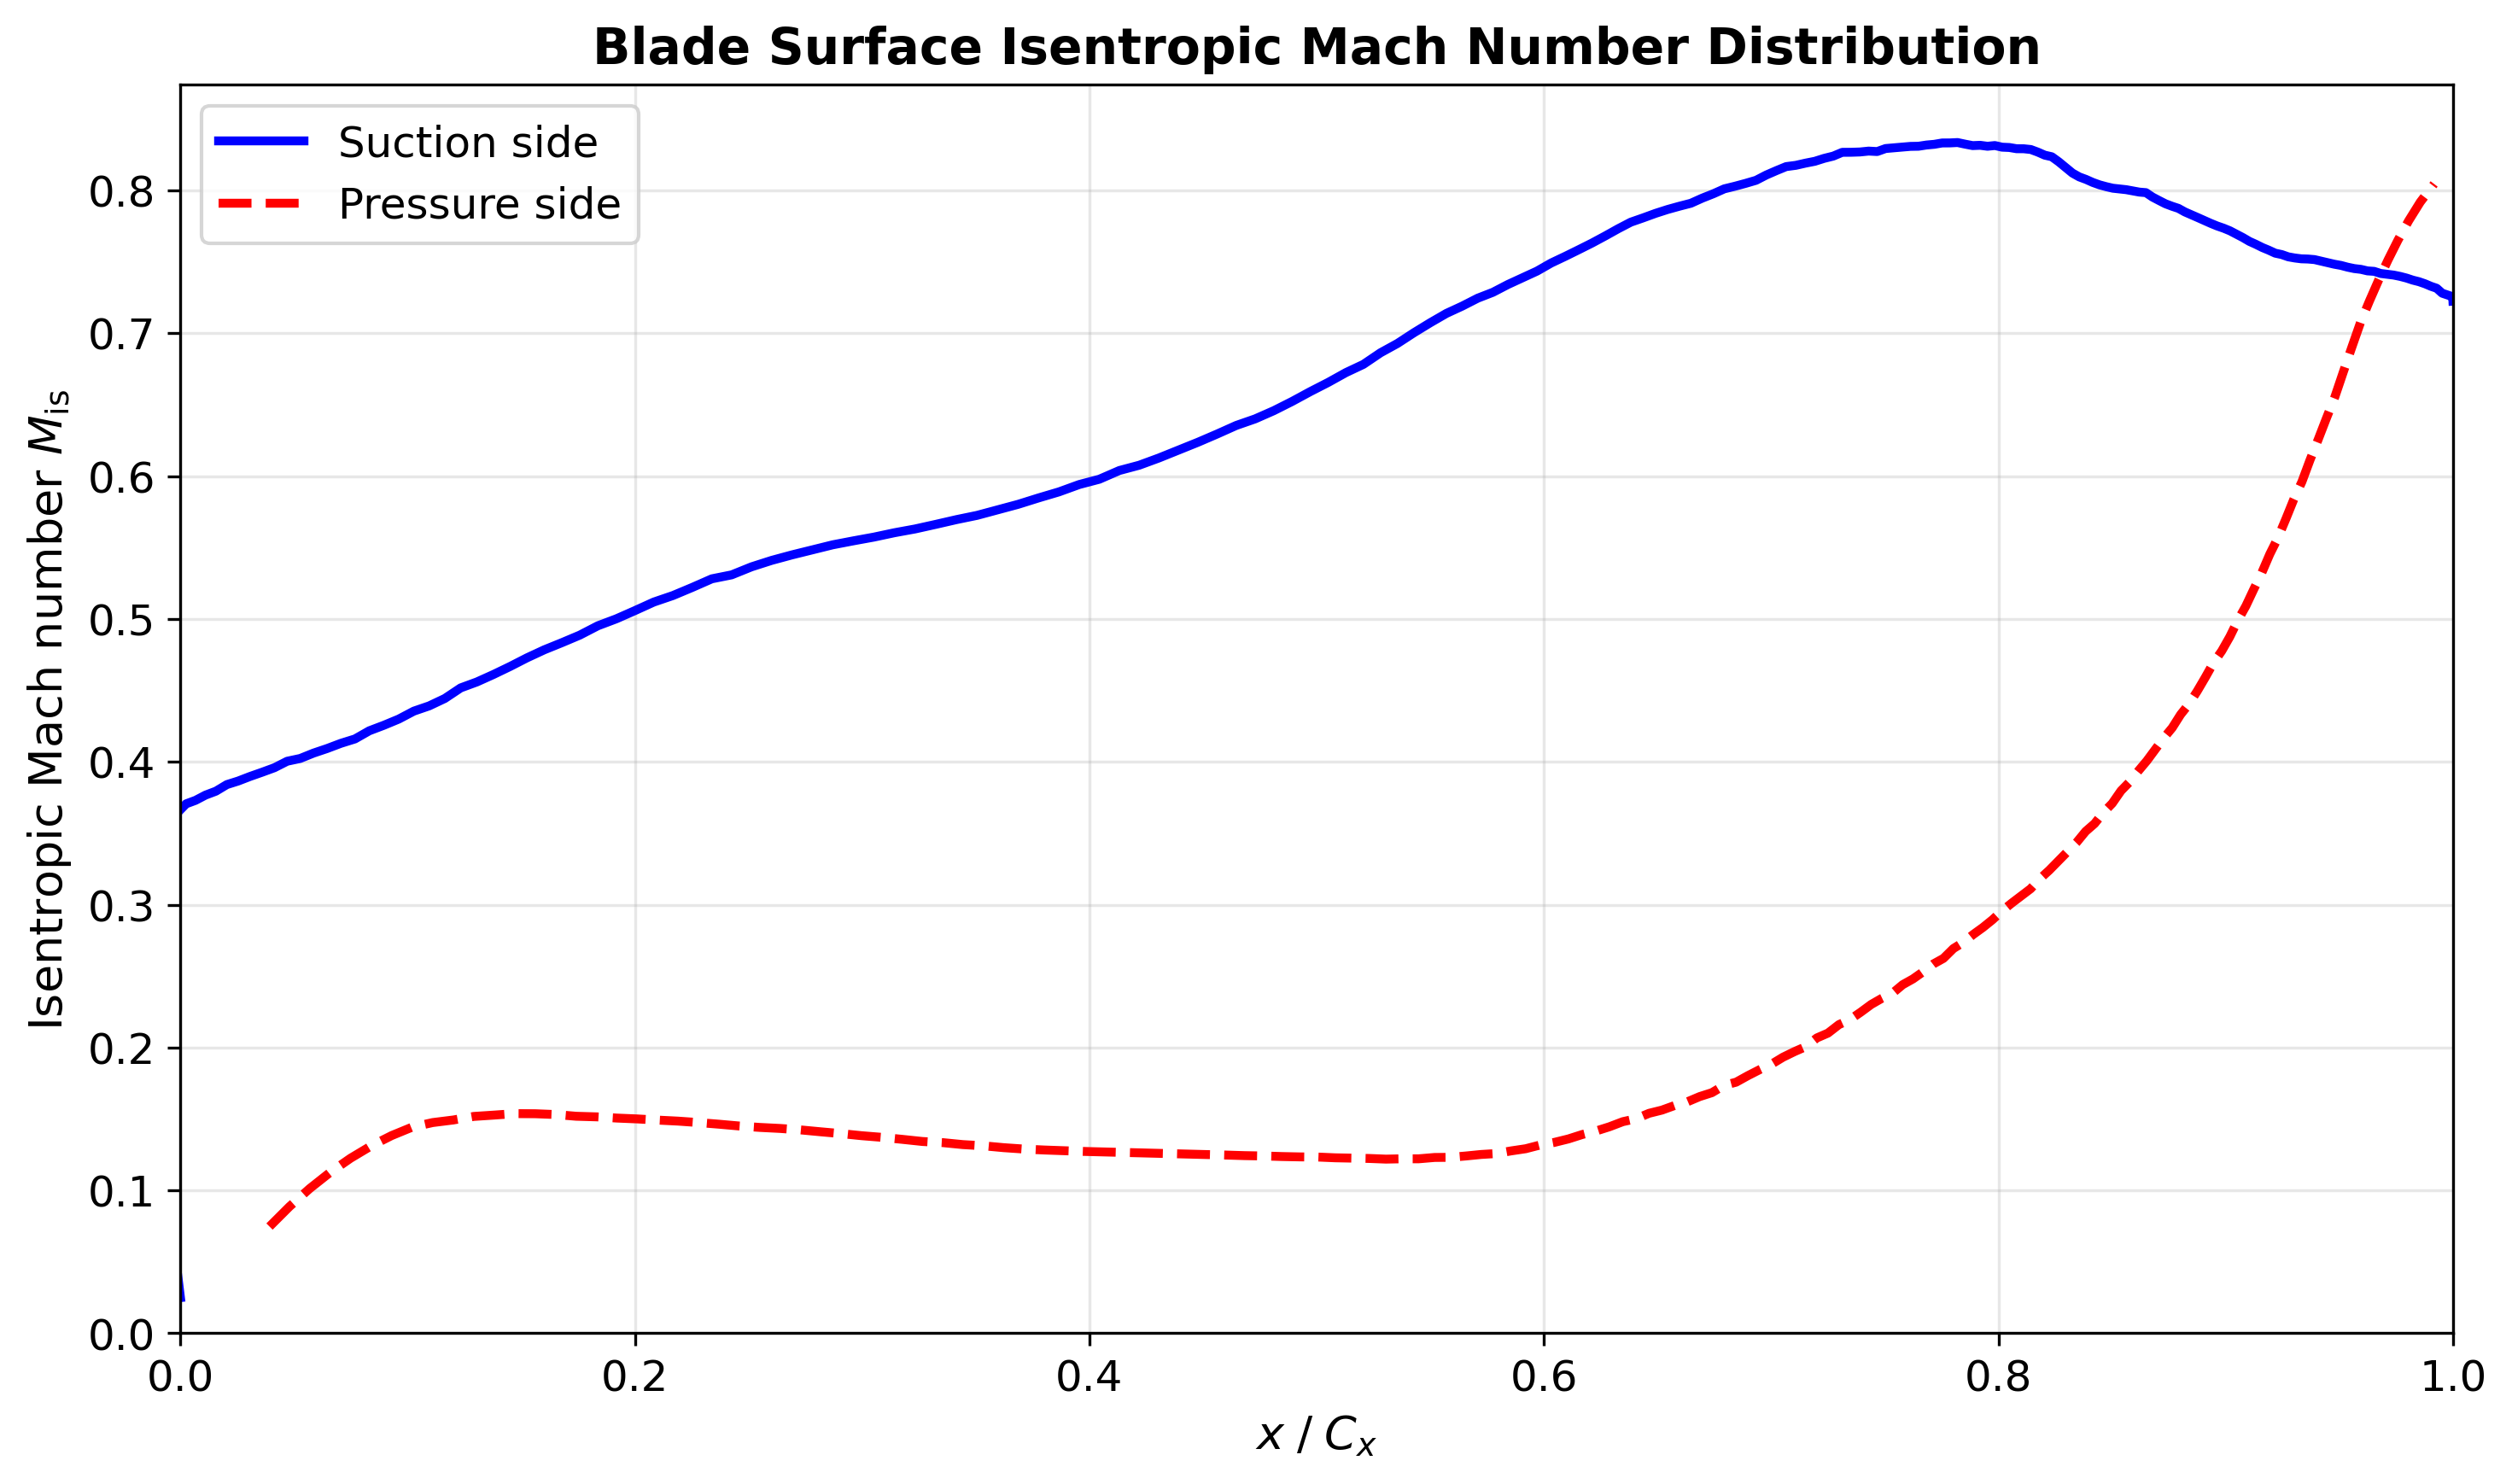
\includegraphics[width=\textwidth]{Isentropic_Mach.png}
    \caption{Isentropic Mach number.}
\end{subfigure}\hfill
\begin{subfigure}{0.48\textwidth}
    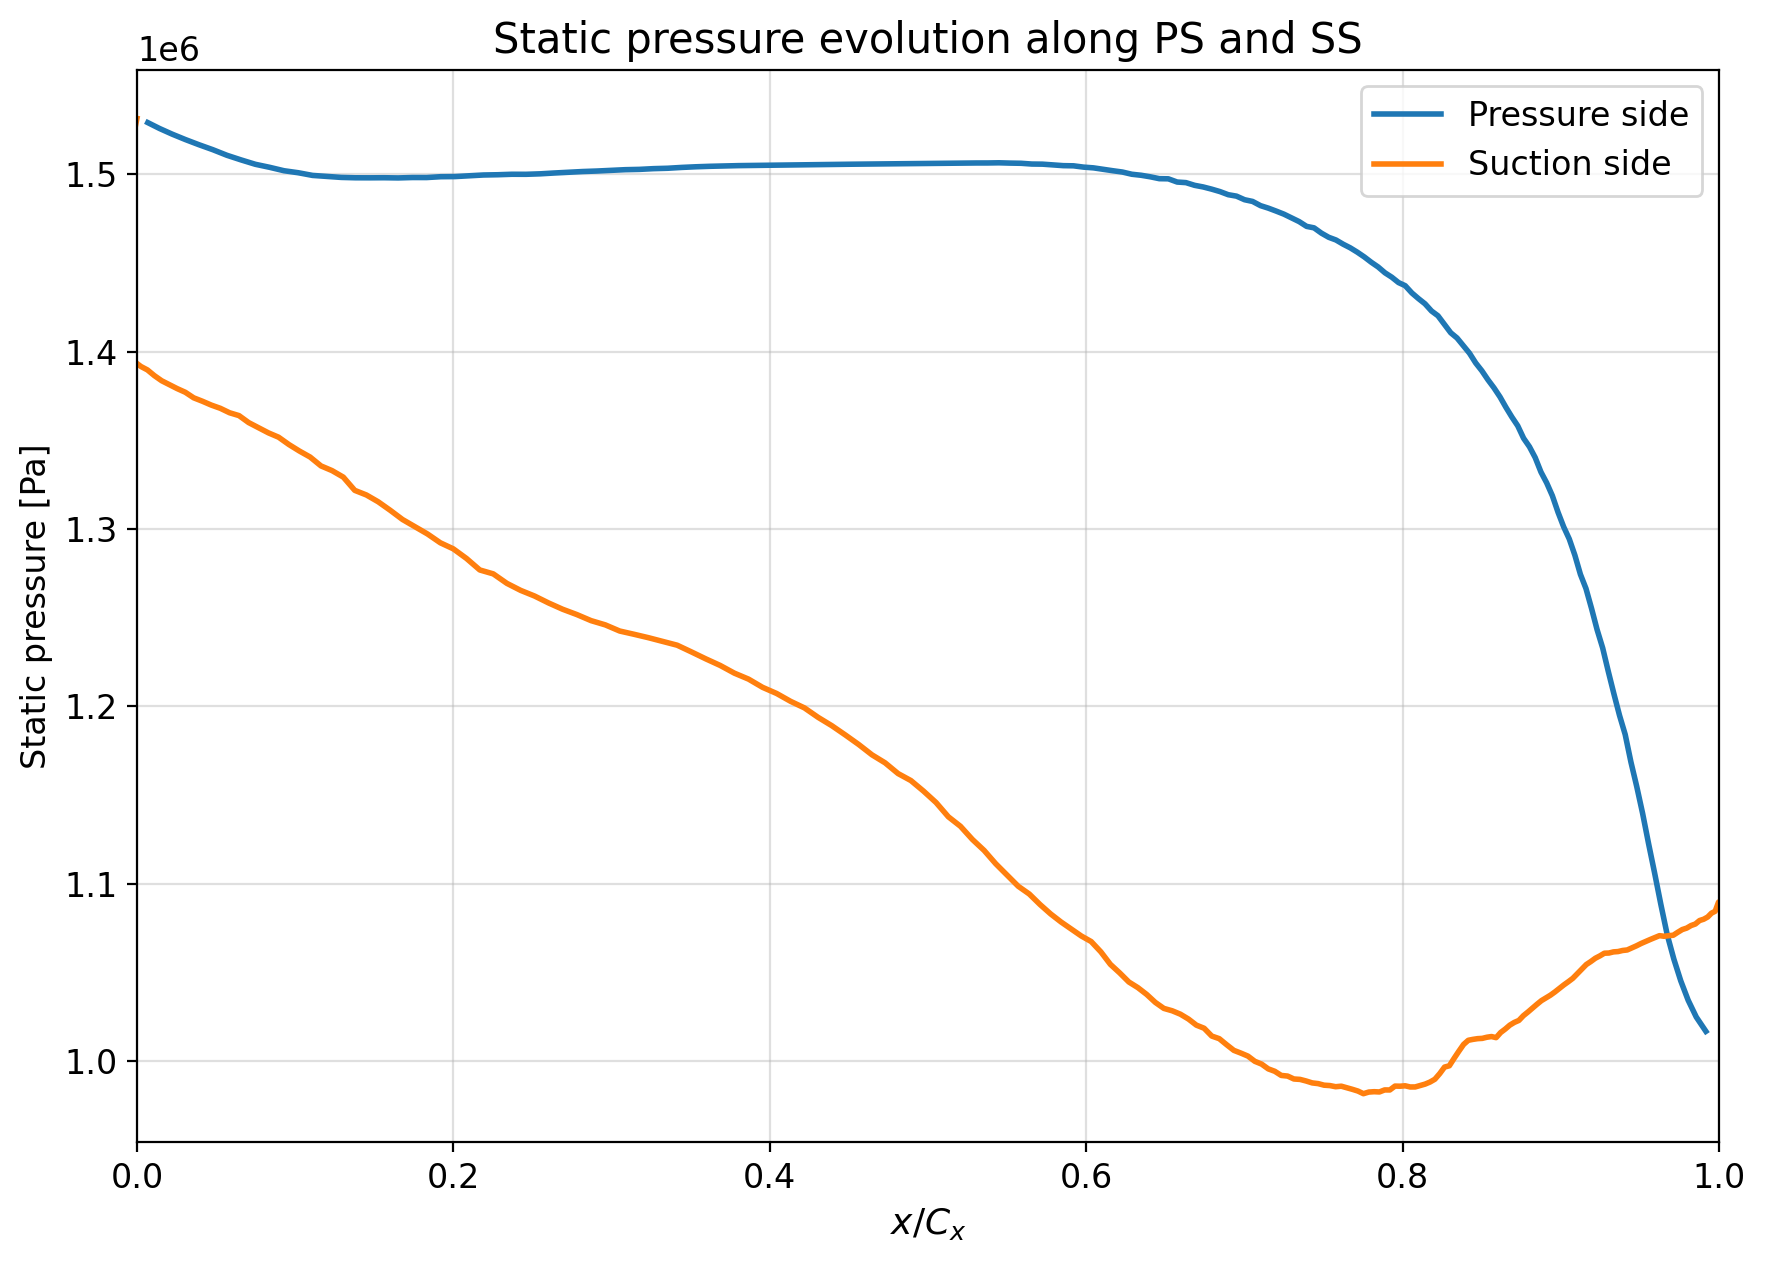
\includegraphics[width=\textwidth]{Pressure Distribution.png}
    \caption{Static pressure on PS / SS.}
\end{subfigure}
\caption{Blade loading: isentropic Mach and static-pressure distribution.}
\label{fig:loading}
\end{figure}

% =====================================================================
\section{Colourmaps of the CFD Analysis}

The Mach-number and static-pressure fields (Fig.~\ref{fig:colourmaps}) show the
flow accelerating through the converging passage, the peak velocity on the
suction side near the throat, and the smooth pressure relaxation towards the
outlet, consistent with the prescribed expansion to $P_3$.

\begin{figure}[H]
\centering
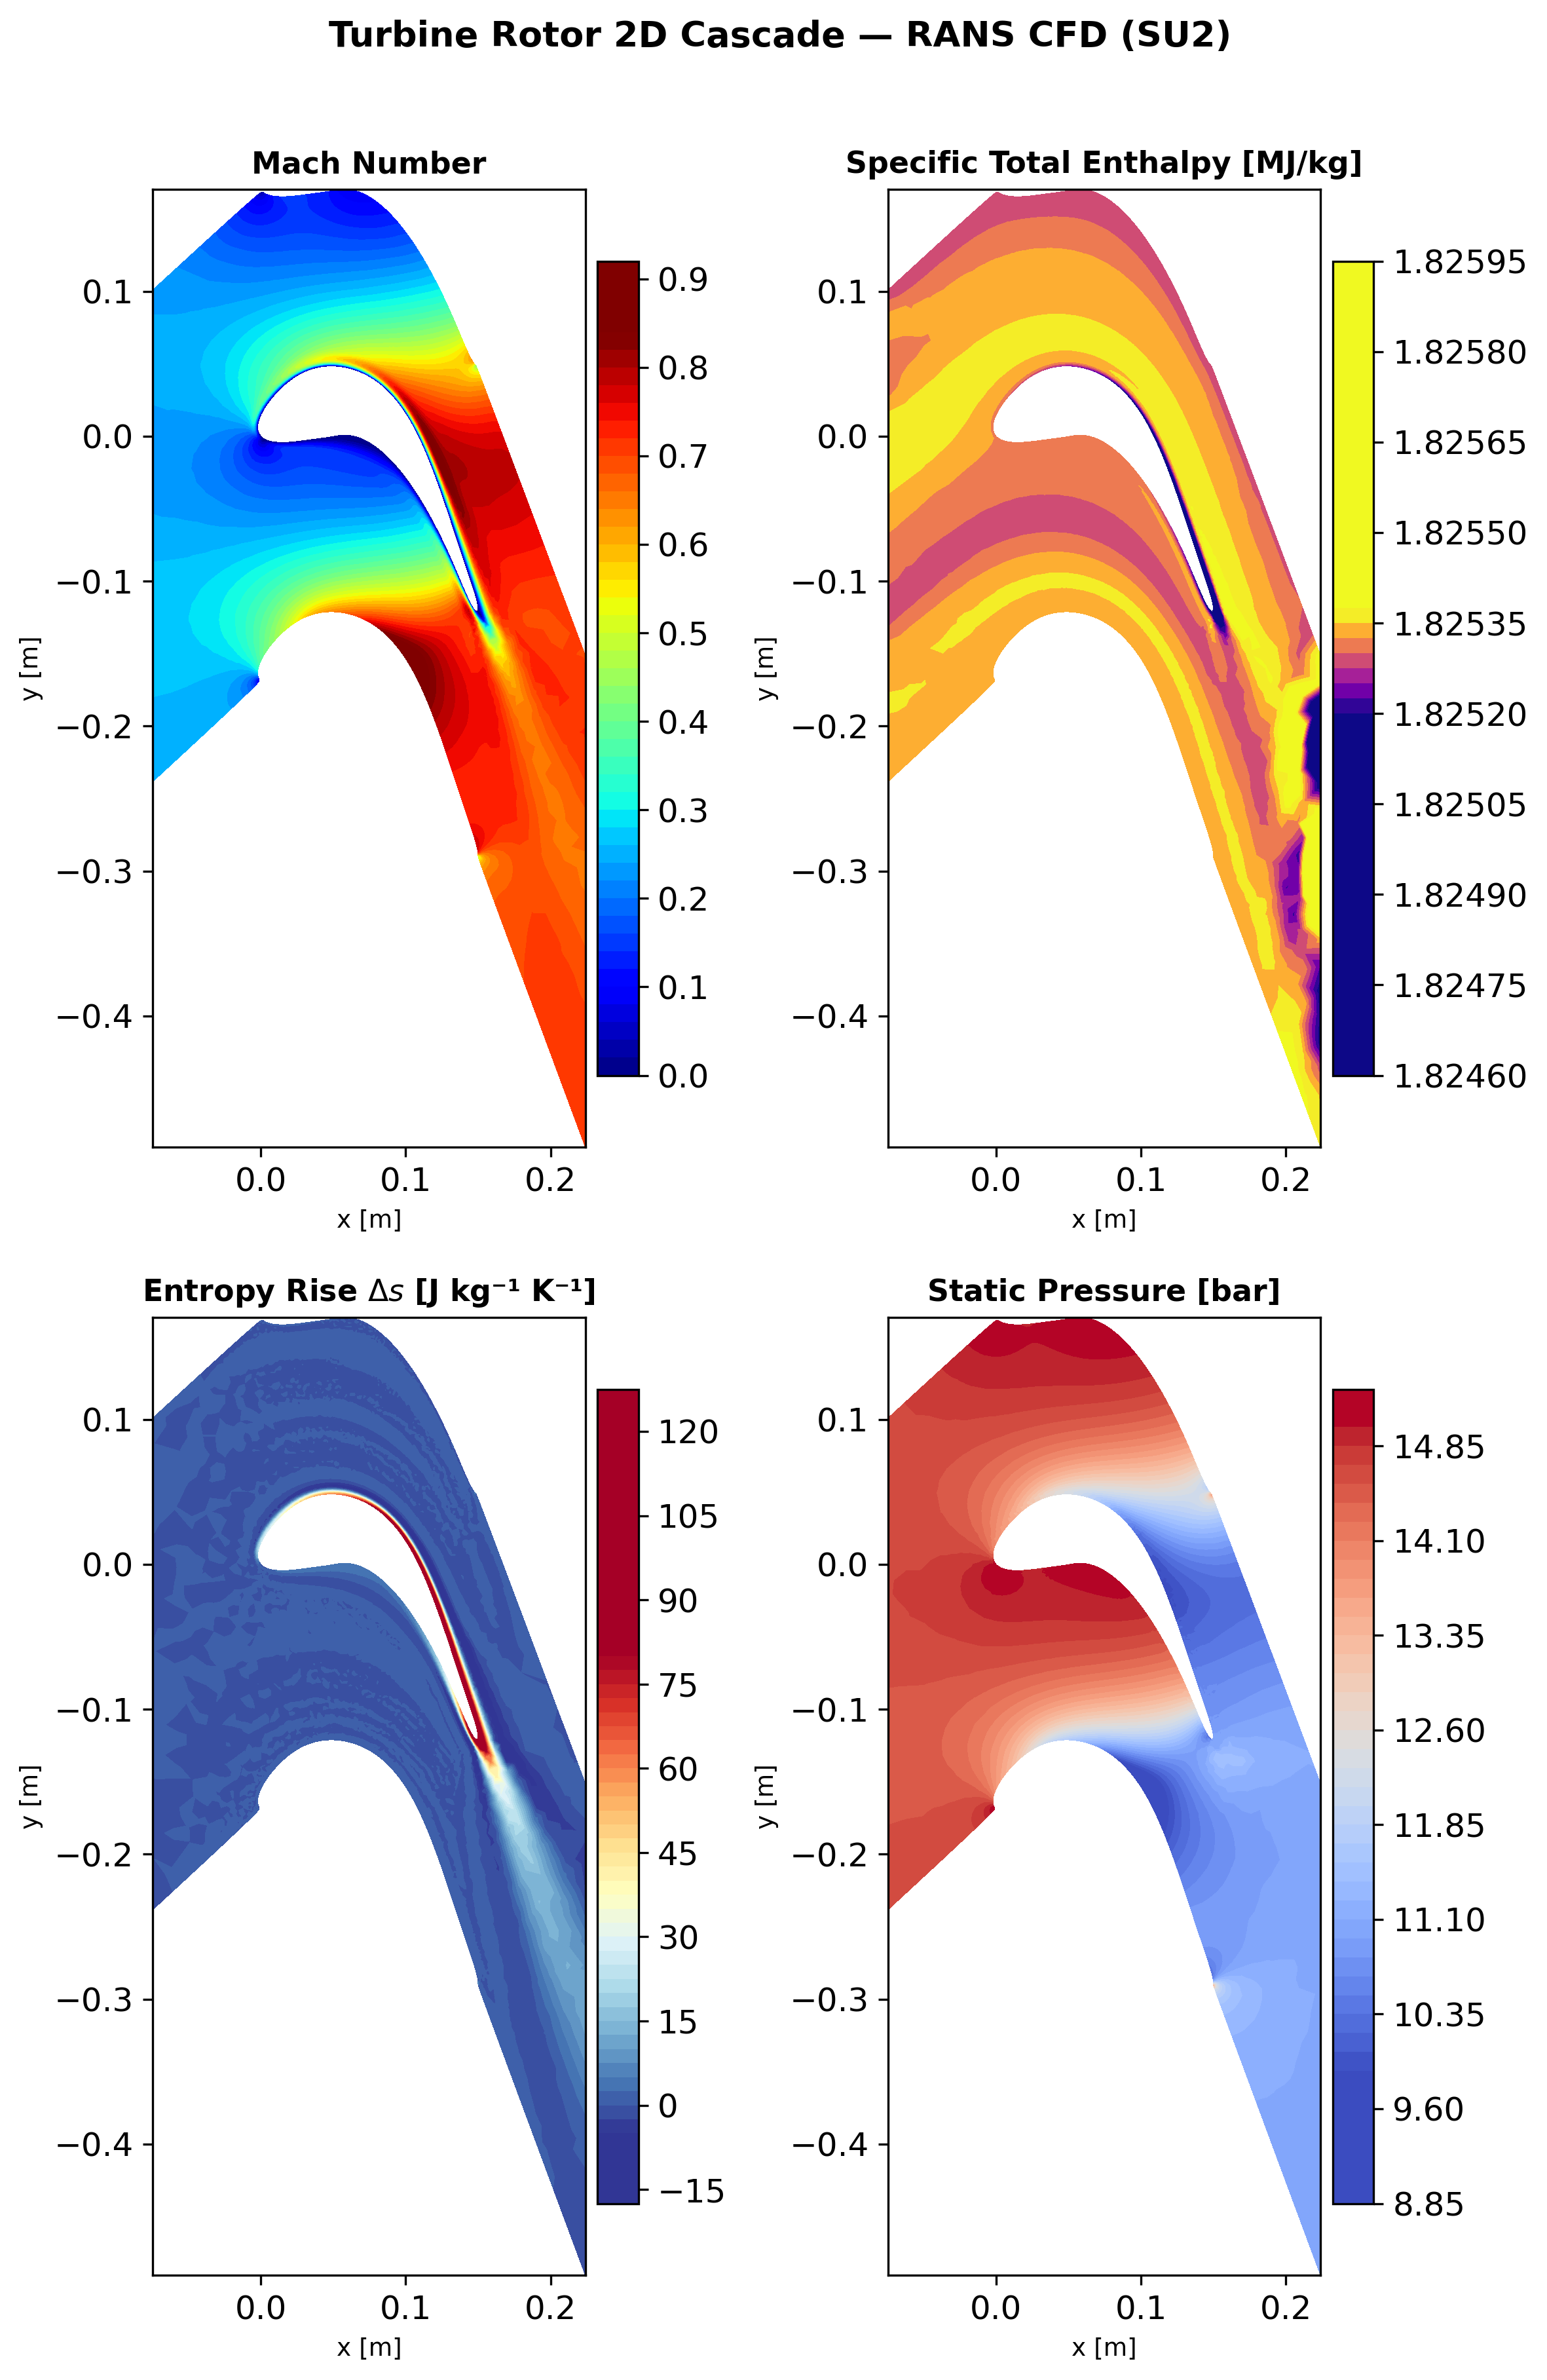
\includegraphics[width=0.95\textwidth]{CFD_Colormaps.png}
\caption{CFD colourmaps of the cascade flow: Mach number, specific total
enthalpy, entropy rise and static pressure.}
\label{fig:colourmaps}
\end{figure}

% =====================================================================
\section{Velocity Profile and Wake}

The pitchwise distributions one trailing-edge region downstream
(Fig.~\ref{fig:wake}) reveal the blade wake as a momentum deficit in all four
quantities -- total pressure, Mach number, flow angle and axial velocity. At the
extraction plane $x = x_{TE}+0.30\,c_x = \SI{0.194}{m}$ the mass-averaged total
pressure is $P_t = \SI{1.49}{MPa}$ ($P_t/P_{t0}=0.978$), the mean Mach number is
$0.681$ and the mean flow angle is $-70.7\degr$. The axial velocity drops from
$\approx \SI{191}{m/s}$ in the free stream to $\approx \SI{158}{m/s}$ in the wake
core (a $9.2\%$ deficit), narrow and well-mixed.

\begin{figure}[H]
\centering
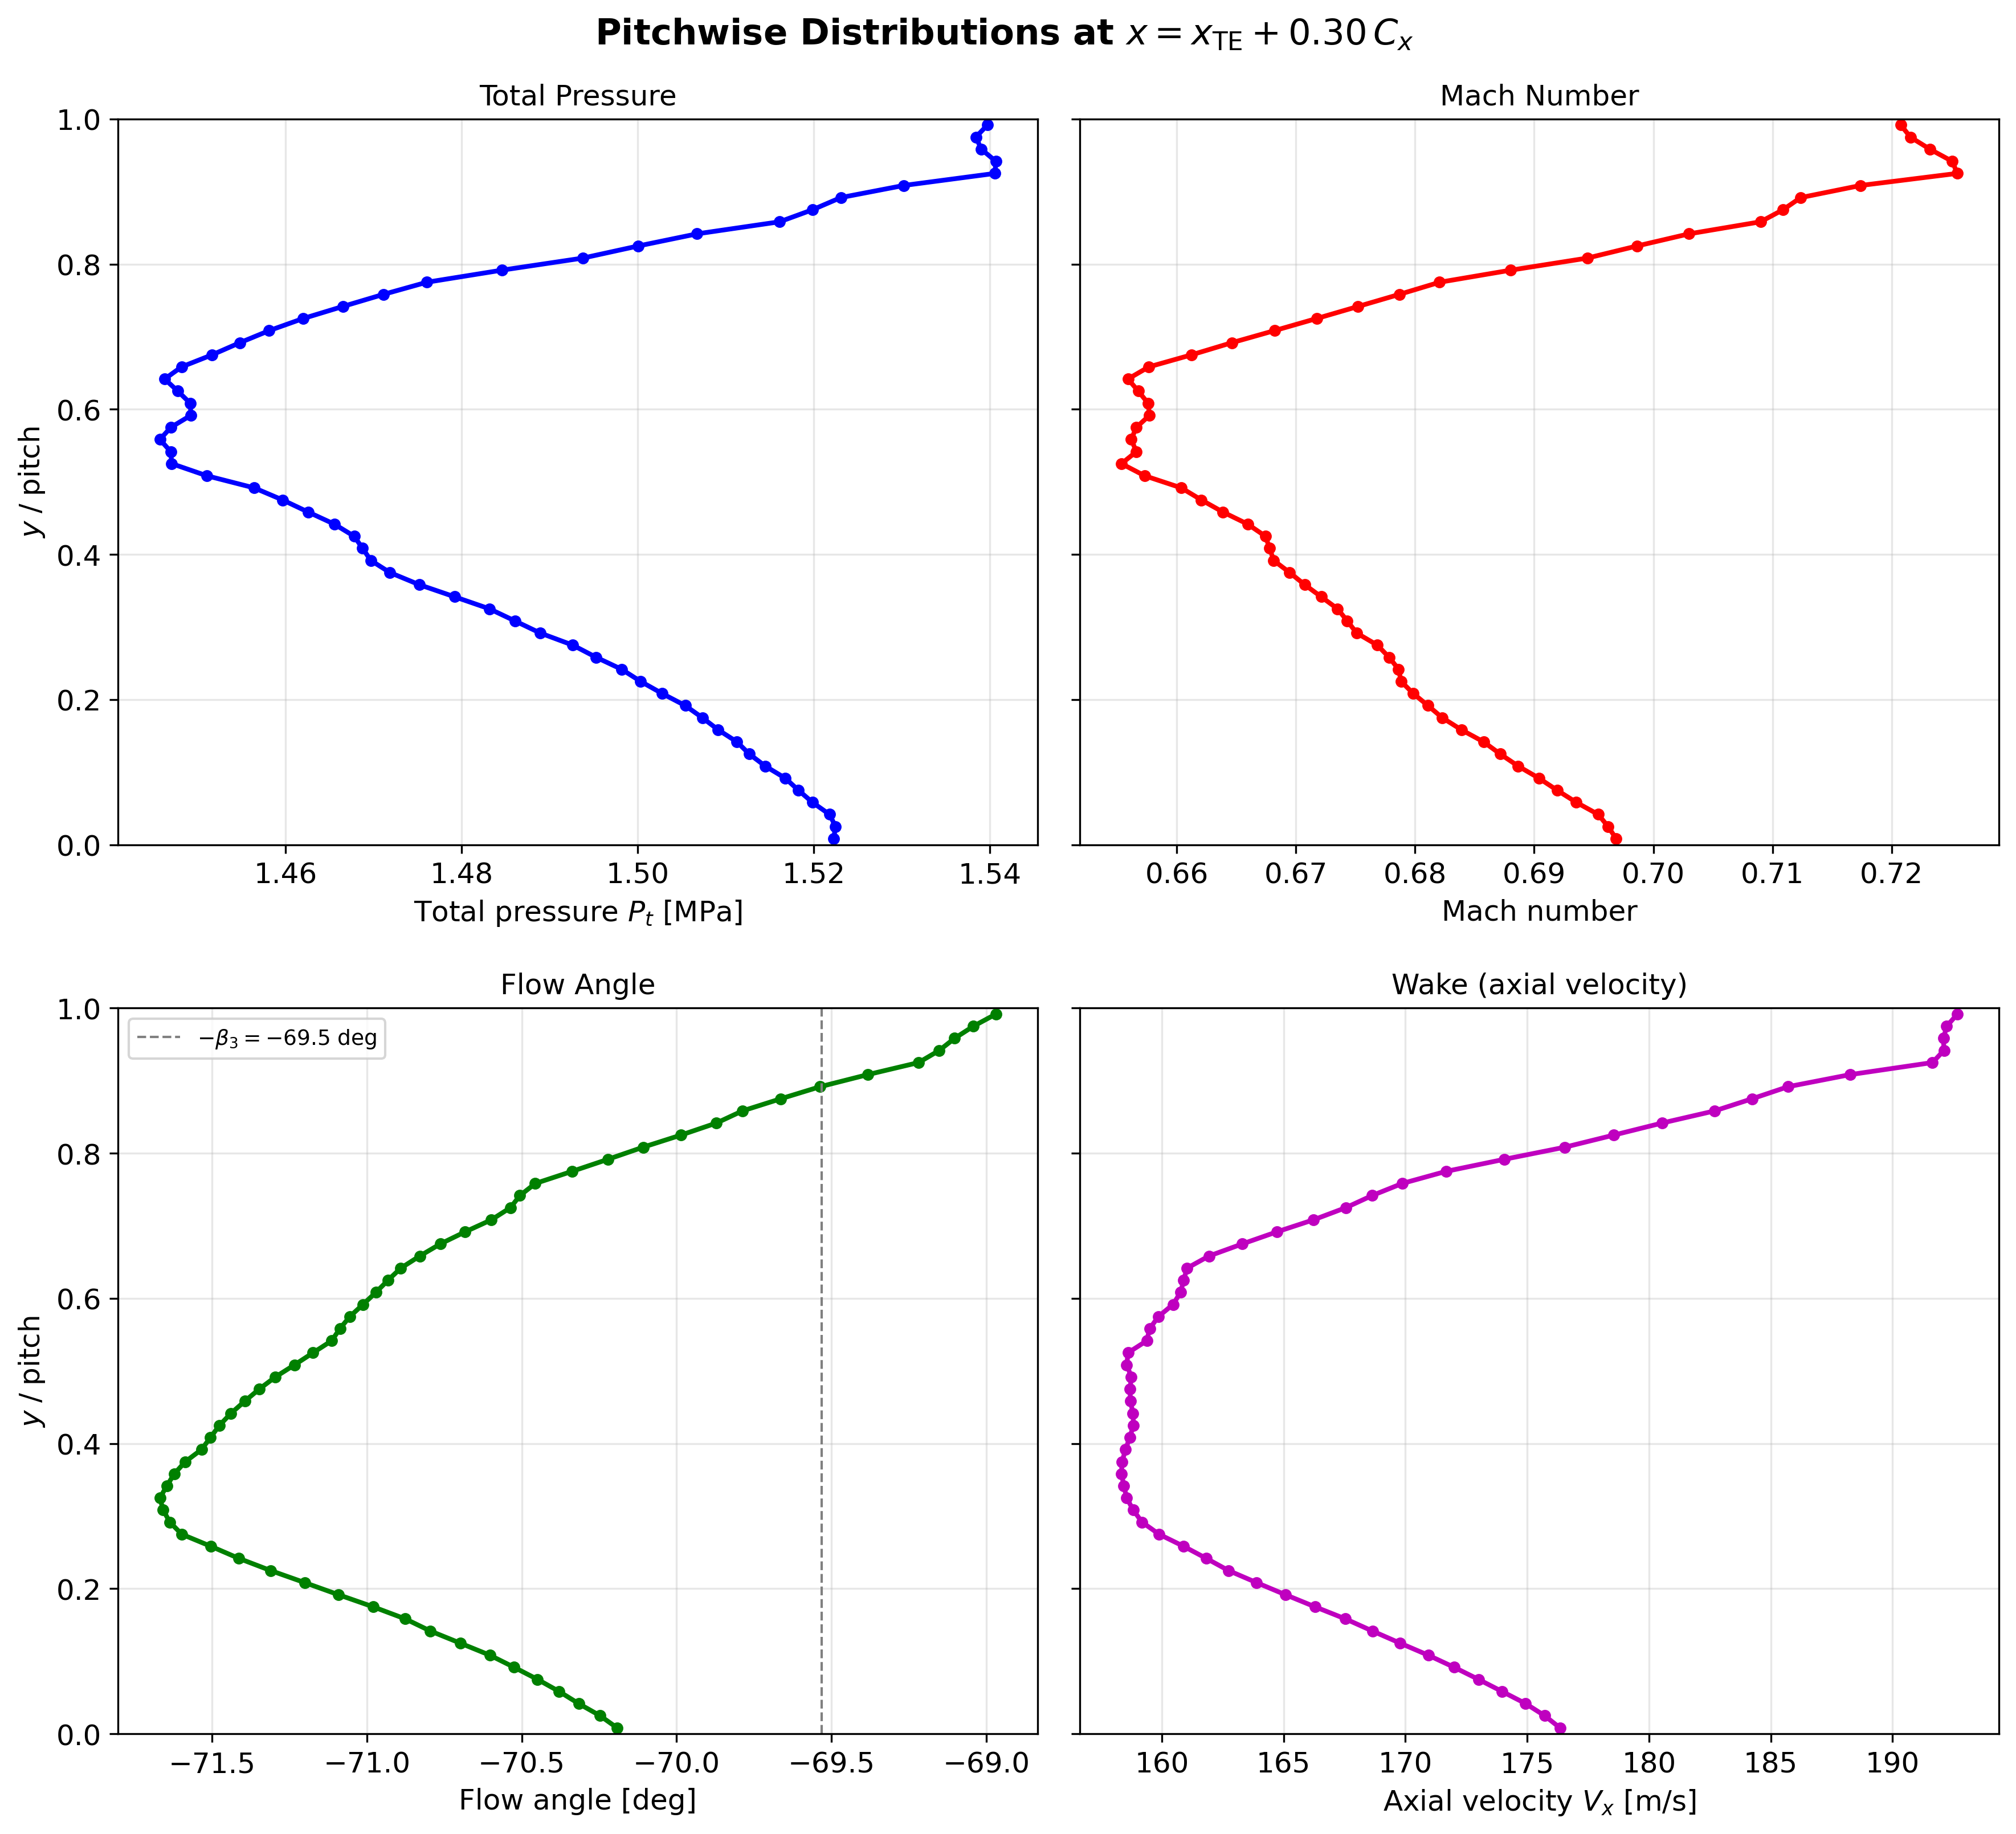
\includegraphics[width=0.88\textwidth]{Pitchwise_Distributions.png}
\caption{Exit-plane pitchwise distributions of total pressure, Mach number, flow
angle and axial velocity (wake), shown un-normalised.}
\label{fig:wake}
\end{figure}

% =====================================================================
\section{CFD Prediction Result}

The CFD confirms the mean-line design: the relative exit Mach number
($M_{w3}\approx 0.67$--$0.68$) and exit angle ($\approx 70\degr$ relative) match
the design intent, the passage delivers the prescribed expansion to $P_3$, and
the stage total-pressure loss across the rotor is modest ($P_t/P_{t0}=0.978$,
i.e.\ $\approx 2.2\%$) with a narrow, attached wake. The blade row is therefore
aerodynamically sound for the chosen mean-line operating point.

% ------------------------------- Chapter 5 -------------------------------
\chapter{Conclusion}

The first stage of a four-stage high-pressure turbine for an F-class industrial
gas turbine (\SI{330}{MW}, \SI{750}{kg/s}, $TIT=\SI{1400}{\degreeCelsius}$) has
been designed through the full preliminary-design chain: 1-D mean-line analysis,
rotor-blade construction and a cascade CFD evaluation.

The mean-line design, closed by a Newton--Raphson iteration on the exit pressure,
delivers the required specific work of \SI{219.27}{kJ/kg} per stage with a blade
speed $U = \SI{349}{m/s}$ at the design coefficients $\psi = 1.8$, $\phi = 0.5$
and $r = 0.35$. The resulting stage has a stator-exit absolute Mach number of
$0.70$, a rotor turning of $112\degr$ and an exit Mach number of $0.30$. Of the
ten design guidelines, eight are met and two ($M_2$ and $h_3/h_2$) are only
marginally violated, so the operating point is essentially feasible and could be
fully cleared by a small adjustment of the coefficients.

The blade row (42 blades, chord \SI{0.192}{m}, stagger $39\degr$, $s/c_x=1.14$)
was constructed with ParaBlade from the metal angles and shown to reproduce the
prescribed curvature. The cascade RANS computation confirms the design: the
loading is smooth and front-loaded, the passage delivers the prescribed expansion
to $P_3 = \SI{1.107}{MPa}$, the relative exit Mach number ($\approx 0.67$) and
exit angle ($\approx 70\degr$) agree with the mean-line prediction, and the rotor
total-pressure loss is modest ($\approx 2.2\%$) with a narrow $9.2\%$ wake
deficit.

Overall, the design is consistent across the three levels of analysis and forms a
sound basis for further refinement (radial equilibrium, cooling, multi-stage
matching and a mesh-independence study of the CFD).


% ------------------------------- Bibliography -------------------------------
\begin{thebibliography}{9}

\bibitem{dixon}
S.~L. Dixon and C.~A. Hall,
\emph{Fluid Mechanics and Thermodynamics of Turbomachinery},
7th ed., Butterworth--Heinemann, 2014.

\bibitem{saravanamuttoo}
H.~Cohen, G.~F.~C. Rogers and H.~I.~H. Saravanamuttoo,
\emph{Gas Turbine Theory}, 6th ed., Pearson Prentice Hall, 2009.

\bibitem{smith}
S.~F. Smith,
``A simple correlation of turbine efficiency,''
\emph{Journal of the Royal Aeronautical Society}, vol.~69, pp.~467--470, 1965.

\bibitem{zweifel}
O.~Zweifel,
``The spacing of turbomachine blading, especially with large angular deflection,''
\emph{Brown Boveri Review}, vol.~32, no.~12, pp.~436--444, 1945.

\bibitem{kacker}
S.~C. Kacker and U.~Okapuu,
``A mean line prediction method for axial flow turbine efficiency,''
\emph{Journal of Engineering for Power}, vol.~104, no.~1, pp.~111--119, 1982.

\bibitem{parablade}
N.~Anand, S.~Vitale, M.~Pini and P.~Colonna,
\emph{ParaBlade: a general parametrization tool for turbomachinery blades},
Delft University of Technology, \url{https://github.com/NAnand-TUD/parablade}.

\bibitem{su2}
T.~D. Economon, F.~Palacios, S.~R. Copeland, T.~W. Lukaczyk and J.~J. Alonso,
``SU2: An open-source suite for multiphysics simulation and design,''
\emph{AIAA Journal}, vol.~54, no.~3, pp.~828--846, 2016.

\bibitem{gmsh}
C.~Geuzaine and J.-F. Remacle,
``Gmsh: A 3-D finite element mesh generator with built-in pre- and
post-processing facilities,''
\emph{International Journal for Numerical Methods in Engineering},
vol.~79, no.~11, pp.~1309--1331, 2009.

\end{thebibliography}


\end{document}
